\documentclass[aspectratio=1610]{beamer}
\usepackage[utf8]{inputenc}
% \usepackage{polski}
\usepackage[T1]{fontenc}
\usepackage{tikz}
\usepackage{tikzducks}
% \usetikzlibrary{decorations.pathmorphing}
\usepackage{multimedia}
\usepackage{graphicx}
\usepackage[justification=centering]{caption}
\usepackage{textcomp}
\usepackage{appendixnumberbeamer}
\usepackage{qrcode}
% \usepackage[natbib, language=polish, sorting=none]{biblatex}
% \addbibresource{lio.bib}
\usepackage{hyperref}
%\usepackage[width=\textwidth]{animate}
%\usepackage{chemformula}
\usepackage{sidecap}
\usepackage{multirow}
\usepackage{multicol}
\usepackage{rotating}
\usepackage{anyfontsize} % change font size for semposiwko

\usepackage{physics}
\usepackage{array}
\usepackage{booktabs}
\usepackage{transparent}
% \usepackage{siunitx}
% \usepackage[rightcaption]{sidecap}
\usepackage{eso-pic}

\usepackage{listings}
\lstset{
basicstyle=\small\ttfamily,
columns=flexible,
breaklines=true
}

% \usepackage{emoji}
\usepackage{subcaption}


\usepackage[natbib, sorting=none]{biblatex}
\addbibresource{lio.bib}
\renewcommand*{\bibfont}{\scriptsize}

\usefonttheme[onlymath]{serif}

\usetheme{Szeged}
\usecolortheme{whale}
\setbeamercolor{palette primary}{bg=violet!80!black,fg=white}
\setbeamercolor{palette secondary}{bg=violet!60!black,fg=white}
% \definecolor{deepviolet}{RGB}{46,0,79}
% \definecolor{vividpink}{RGB}{255,0,127}
% \setbeamercolor{palette primary}{bg=deepviolet,fg=white}
% \setbeamercolor{palette secondary}{bg=vividpink,fg=white}
\setbeamercolor{palette tertiary}{bg=violet!40!black,fg=white}
\setbeamercolor{palette quaternary}{bg=violet!20!black,fg=white}
\setbeamercolor{structure}{fg=violet!60!black}
\setbeamertemplate{caption}{\insertcaption}
% \setbeamertemplate{headline}{
%   \begin{beamercolorbox}[wd=.9\paperwidth]{headline}
%     \vspace{1.5ex}
%     \insertsectionnavigationhorizontal
%     \vspace{1.5ex}
%   \end{beamercolorbox}
% }
% \definecolor{violet-dark}{HTML}{4B0082}
% \definecolor{teal}{HTML}{008080}
% \definecolor{amber}{HTML}{FFC107}
% \definecolor{light-grey}{HTML}{F5F5F5}
% \definecolor{charcoal}{HTML}{333333}
% \setbeamercolor{palette primary}{bg=violet-dark, fg=white}
% \setbeamercolor{palette secondary}{bg=teal, fg=white}
% \setbeamercolor{palette tertiary}{bg=amber, fg=charcoal}
% \setbeamercolor{background canvas}{bg=light-grey}
% \setbeamercolor{normal text}{fg=charcoal}
% Główna paleta fioletów
% \definecolor{coolblack}{HTML}{000000}
% \definecolor{coolnavy}{HTML}{14213D}
% \definecolor{coolorange}{HTML}{FCA311}
% \definecolor{coollightgray}{HTML}{E5E5E5}
% \definecolor{coolwhite}{HTML}{FFFFFF}

% % Opcjonalnie: ustawienia kolorów dla Beamera
% \setbeamercolor{normal text}{fg=coolblack,bg=coolwhite}
% \setbeamercolor{structure}{fg=coolorange}
% \setbeamercolor{frametitle}{fg=coolwhite,bg=coolnavy}
% \setbeamercolor{title}{fg=coolwhite,bg=coolnavy}
% \setbeamercolor{item}{fg=coolorange}
% \setbeamercolor{block title}{fg=coolwhite,bg=coolnavy}
% \setbeamercolor{block body}{fg=coolblack,bg=coollightgray}
% \setbeamercolor{palette tertiary}{fg=coolwhite, bg=coolorange}
% \setbeamercolor{palette quaternary}{fg=coolblack, bg=coollightgray}

\linespread{0.8}

\setbeamertemplate{background}%
{%
    \begin{tikzpicture}[remember picture,overlay]{\node[yshift=1.5cm,xshift=-2cm,opacity=0.1] at (current page.south east)
      {
      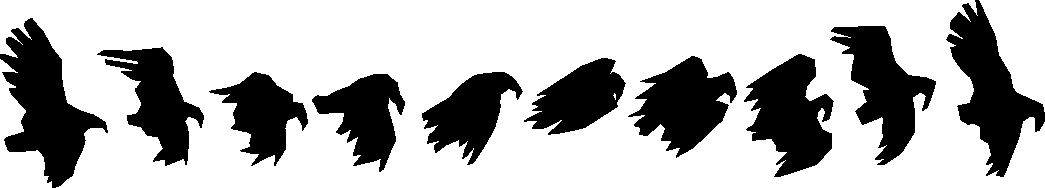
\includegraphics[scale=0.4, angle=25]{ptaki.pdf}
      }
      ;
    \node[yshift=-2cm,xshift=-2cm,opacity=0.1] at (current page.north east)
      {
      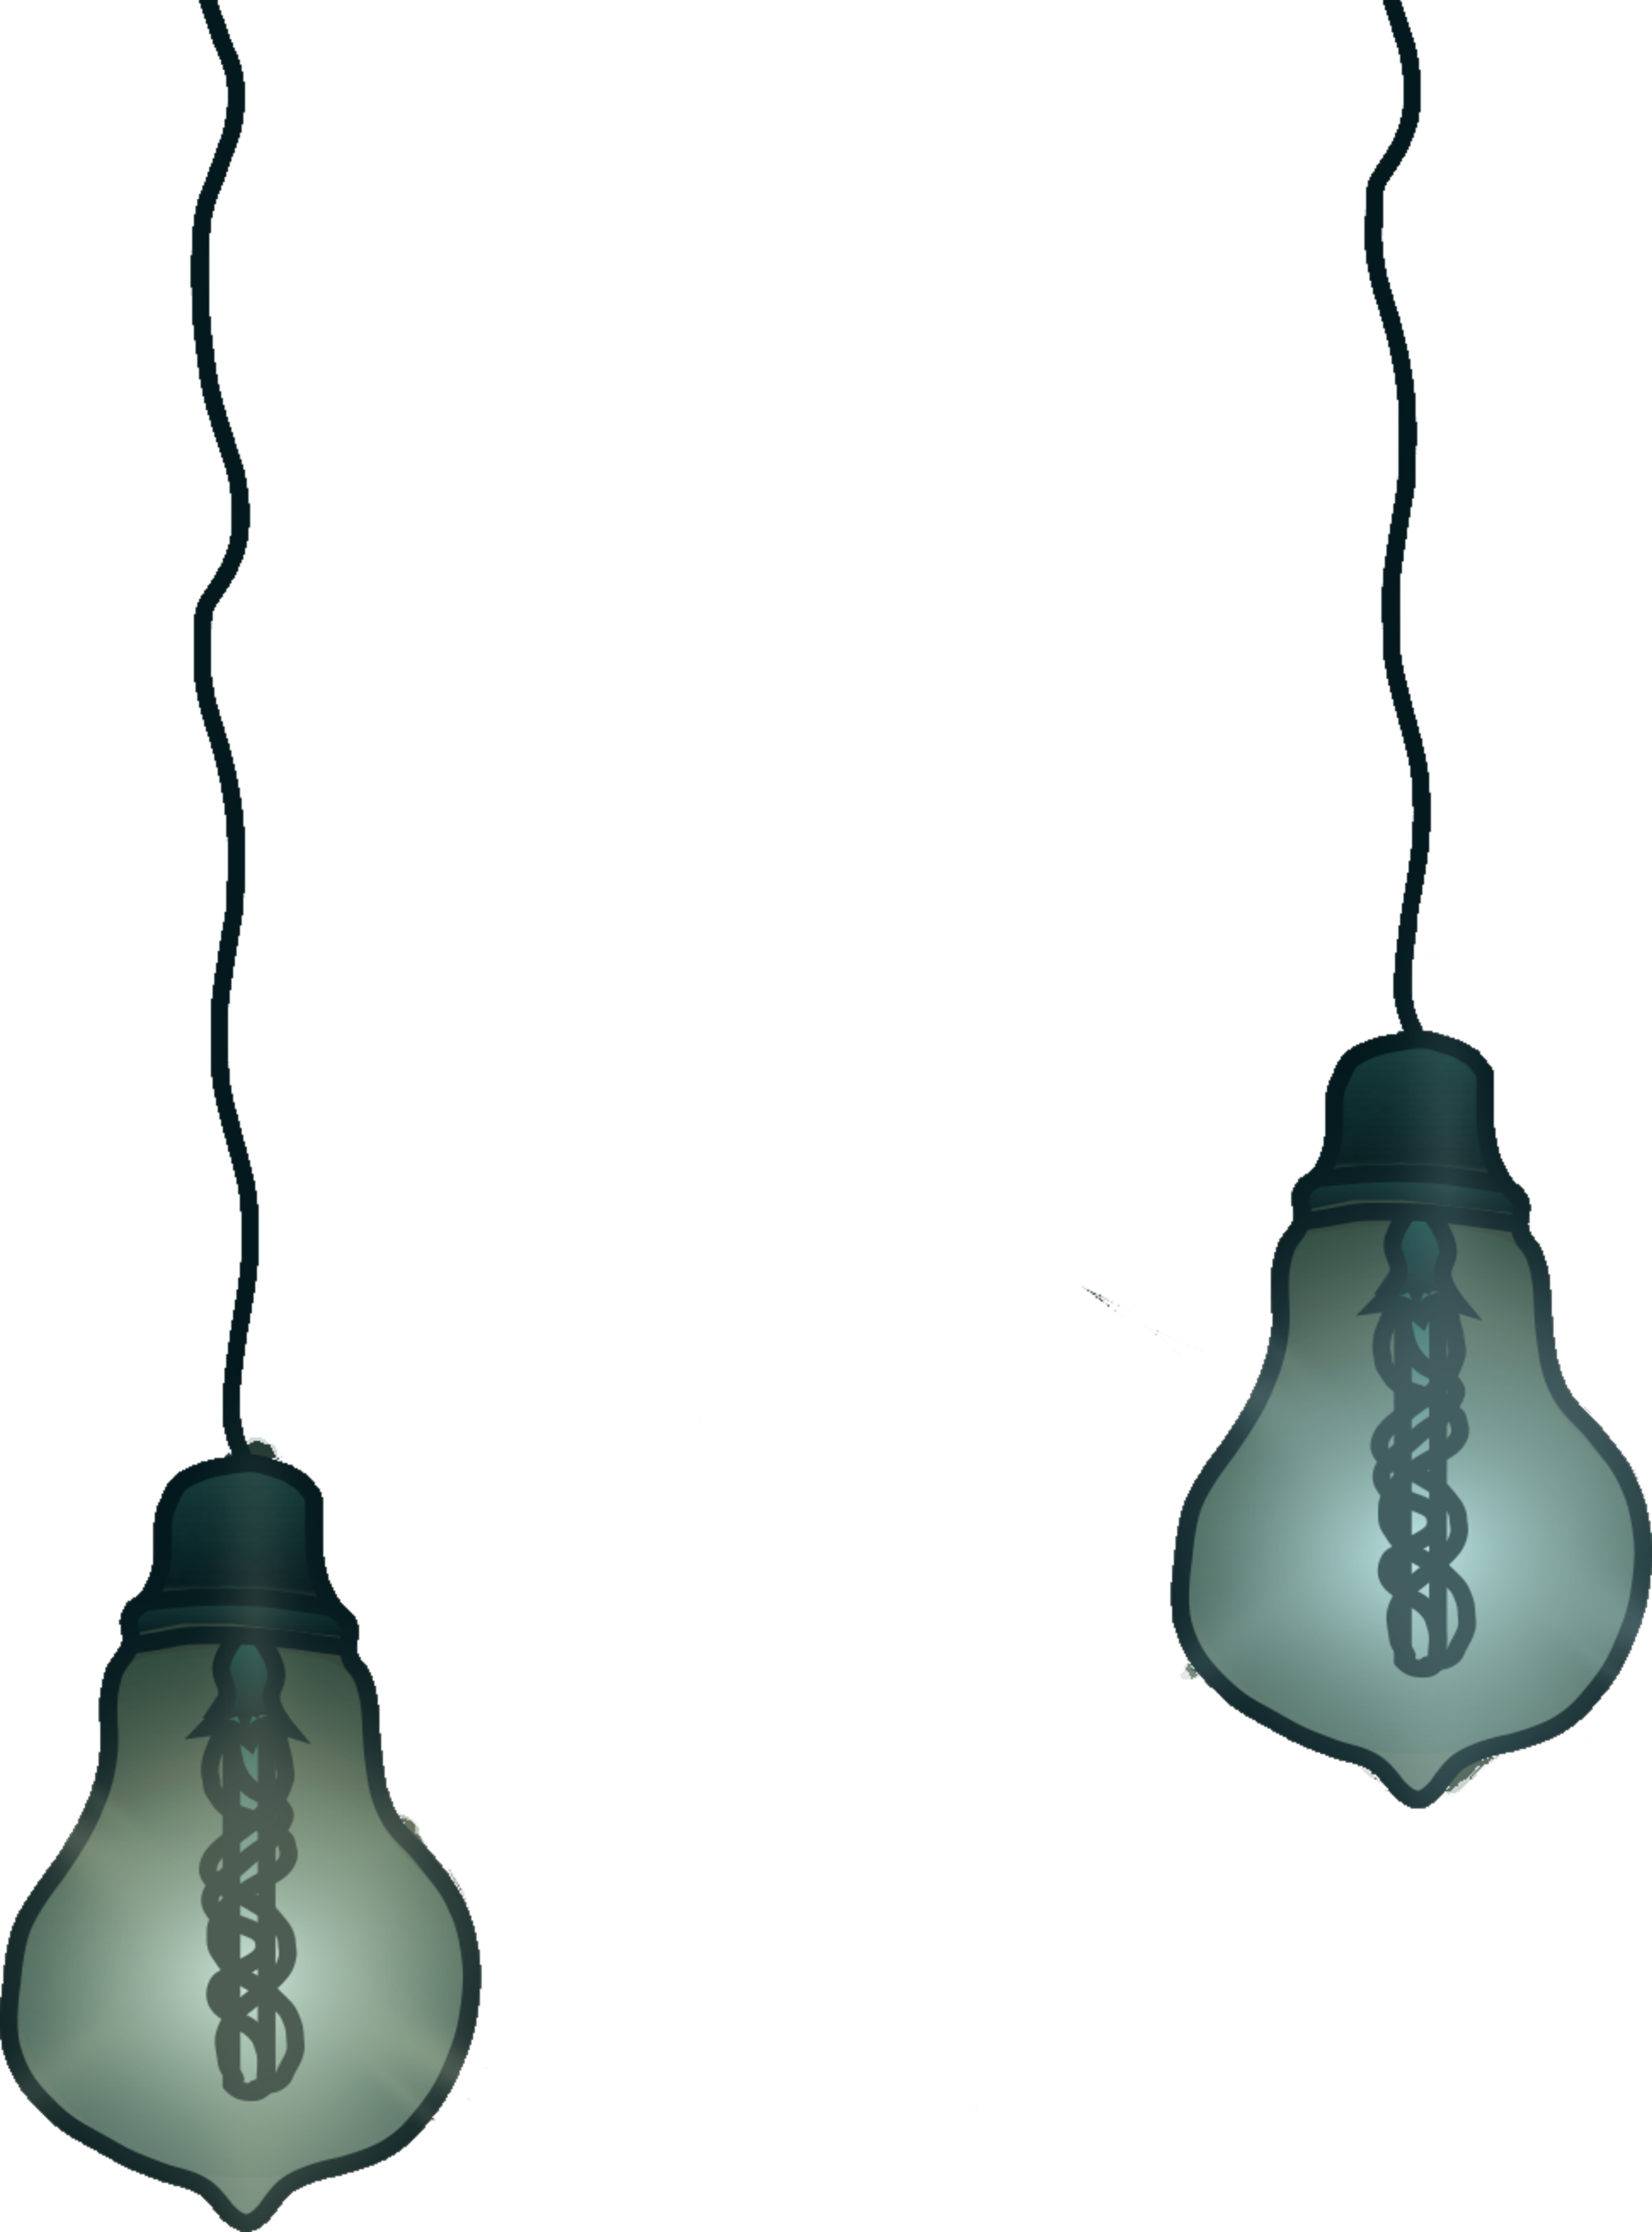
\includegraphics[scale=0.1, angle=0]{zarowki.pdf}
      }
      ;
    \node[yshift=1.0cm,xshift=0.6cm] (logopos) at (current page.south west) {{\begin{tikzpicture}\shuffleducks\duck[signpost=\insertframenumber, \randomhead,scale=.4]\end{tikzpicture}}};
    \pgfmathsetmacro{\progress}{360*(\insertframenumber)/(\inserttotalframenumber)};
    \draw[line width=0.2*3pt] ([xshift=0.55cm] logopos)  arc[radius=0.55cm, start angle=0, end angle=\progress];
    \fill ([shift={(\progress:0.55cm)}] logopos) circle(1pt);

    }
        \end{tikzpicture}
    
}

\newcommand{\SeMPowisko}{%
\large S\normalsize%
\kern-.3em \lower.2ex\hbox{e}%
\lower.2ex\hbox{\large M\normalsize}%
\kern-.1em \raise.1ex\hbox{\large P\normalsize}%
\kern-.3em \lower.2ex\hbox{o}%
\kern-.2em \raise.2ex\hbox{w}%
\lower.2ex\hbox{i}%
s%
\raise.2ex\hbox{k}%
\kern-.3em \lower.2ex\hbox{o}%
}
% \usepackage{microtype}
% \DeclareRobustCommand{\SeMPowisko}{SeMPowisko}


% \newcommand\Tikz{Ti\emph{k}Z}
% \definecolor{neworange}{RGB}{255,140,0}
\renewcommand{\figurename}{figure}


\title[talking with the satellites]{Talking with the Satellites}
\subtitle{Building a Low-Cost Ground Station with SatNOGS}
\author[M. Winiarski]{Mateusz ,,\(\blacksquare\)'' Winiarski}
\institute[kmpsuj, sempowisko]{KMPS UJ \\biophysics, FAIS, Jagiellonian University in Kraków} 
\date[dzisiaj]{\SeMPowisko{} 2025\\today}

\begin{document}

\frame{\titlepage}

\section{hello}

% \subsection{hello}

\begin{frame}{satellite rise}
\begin{figure}
 \centering
 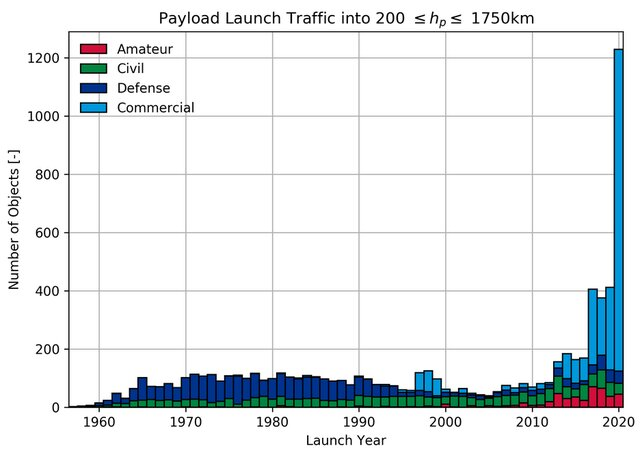
\includegraphics[width=0.7\textwidth]{images/2025-05-23-01-28-10.png}
 \caption{number of satellites launched yearly into LEO (low earth orbit)}
 \end{figure}
\end{frame}

\begin{frame}{can i launch a satellite?}
\begin{columns}
\column{0.5\textwidth}
\begin{figure}
 \centering
 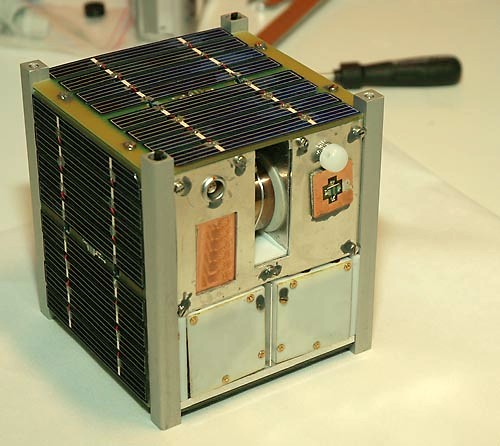
\includegraphics[width=0.9\textwidth]{images/2025-05-22-16-14-36.png}
 \caption{a cubesat}
 \end{figure}

\column{0.5\textwidth}
\begin{figure}
 \centering
 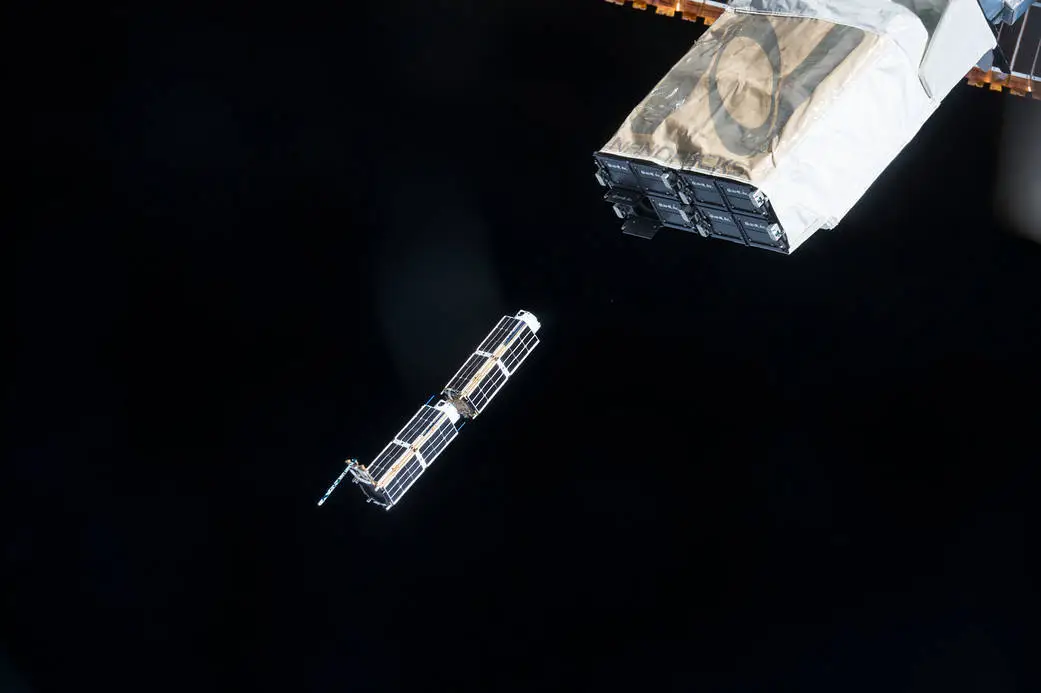
\includegraphics[width=0.9\textwidth]{images/2025-05-22-16-16-01.png}
 \caption{a cubesat deployer}
 \end{figure}
\end{columns}
\end{frame}

\begin{frame}{motivation}{}

% TikZ illustration: Satellite in LEO transmitting telemetry to Earth station (motivation slide)
\begin{tikzpicture}[scale=1.0, every node/.style={font=\sffamily}, >=latex]
  % Earth
  \shade[ball color=blue!40!black] (0,0) circle (2);
  \node[white] at (0,0) {Earth};

  % Ground station (simple antenna)
  \draw[fill=gray!40] (-1.5,-2) -- (-1.3,-1.7) -- (-1.7,-1.7) -- cycle;
  \draw[line width=0.5pt] (-1.5,-1.7) -- ++(-0.5,0.5);
  \draw[line width=0.5pt] (-1.5,-1.7) -- ++(0.5,0.5);
  \node at (-1.5,-2.3) {ground station};

  % Satellite orbit
  \draw[dashed, black, line width=0.5pt] (3,0) arc[start angle=0, end angle=180, radius=3];

  % Satellite
  \begin{scope}[xshift=2cm, yshift=2cm]
    \draw[fill=gray!80] (0,0) rectangle (0.6,0.3);
    \draw (0.3,0.15) -- ++(0.7,0) node[below left] {telemetry};
    \draw[->, thick, red] (0.3,0.15) -- ++(-2.5,-2.5);
    % Antenna on satellite
    \draw[line width=0.3pt] (0.3,0.15) -- ++(0.3,0.3);
    \draw[line width=0.3pt] (0.3,0.15) -- ++(-0.3,0.3);
    \node [above] at (0.3,0.4) {LEO satellite};
  \end{scope}

  % Title
  % \node at (0,2.8) {\Large \textbf{Why Listen to Satellites?}};
\pause
  % Annotation bubble
  \node[align=left, text width=6cm, anchor=west] at (4,-1.5) {
    \textbf{motivation:}\\
    \begin{itemize}[<+->]
      \item access real-time scientific data from space
      \item study RF propagation and satellite orbits
      \item contribute to global open-source networks (SatNOGS)
    \end{itemize}
  };
\end{tikzpicture}



\end{frame}

\begin{frame}{listening to waves}

\begin{figure}
 \centering
 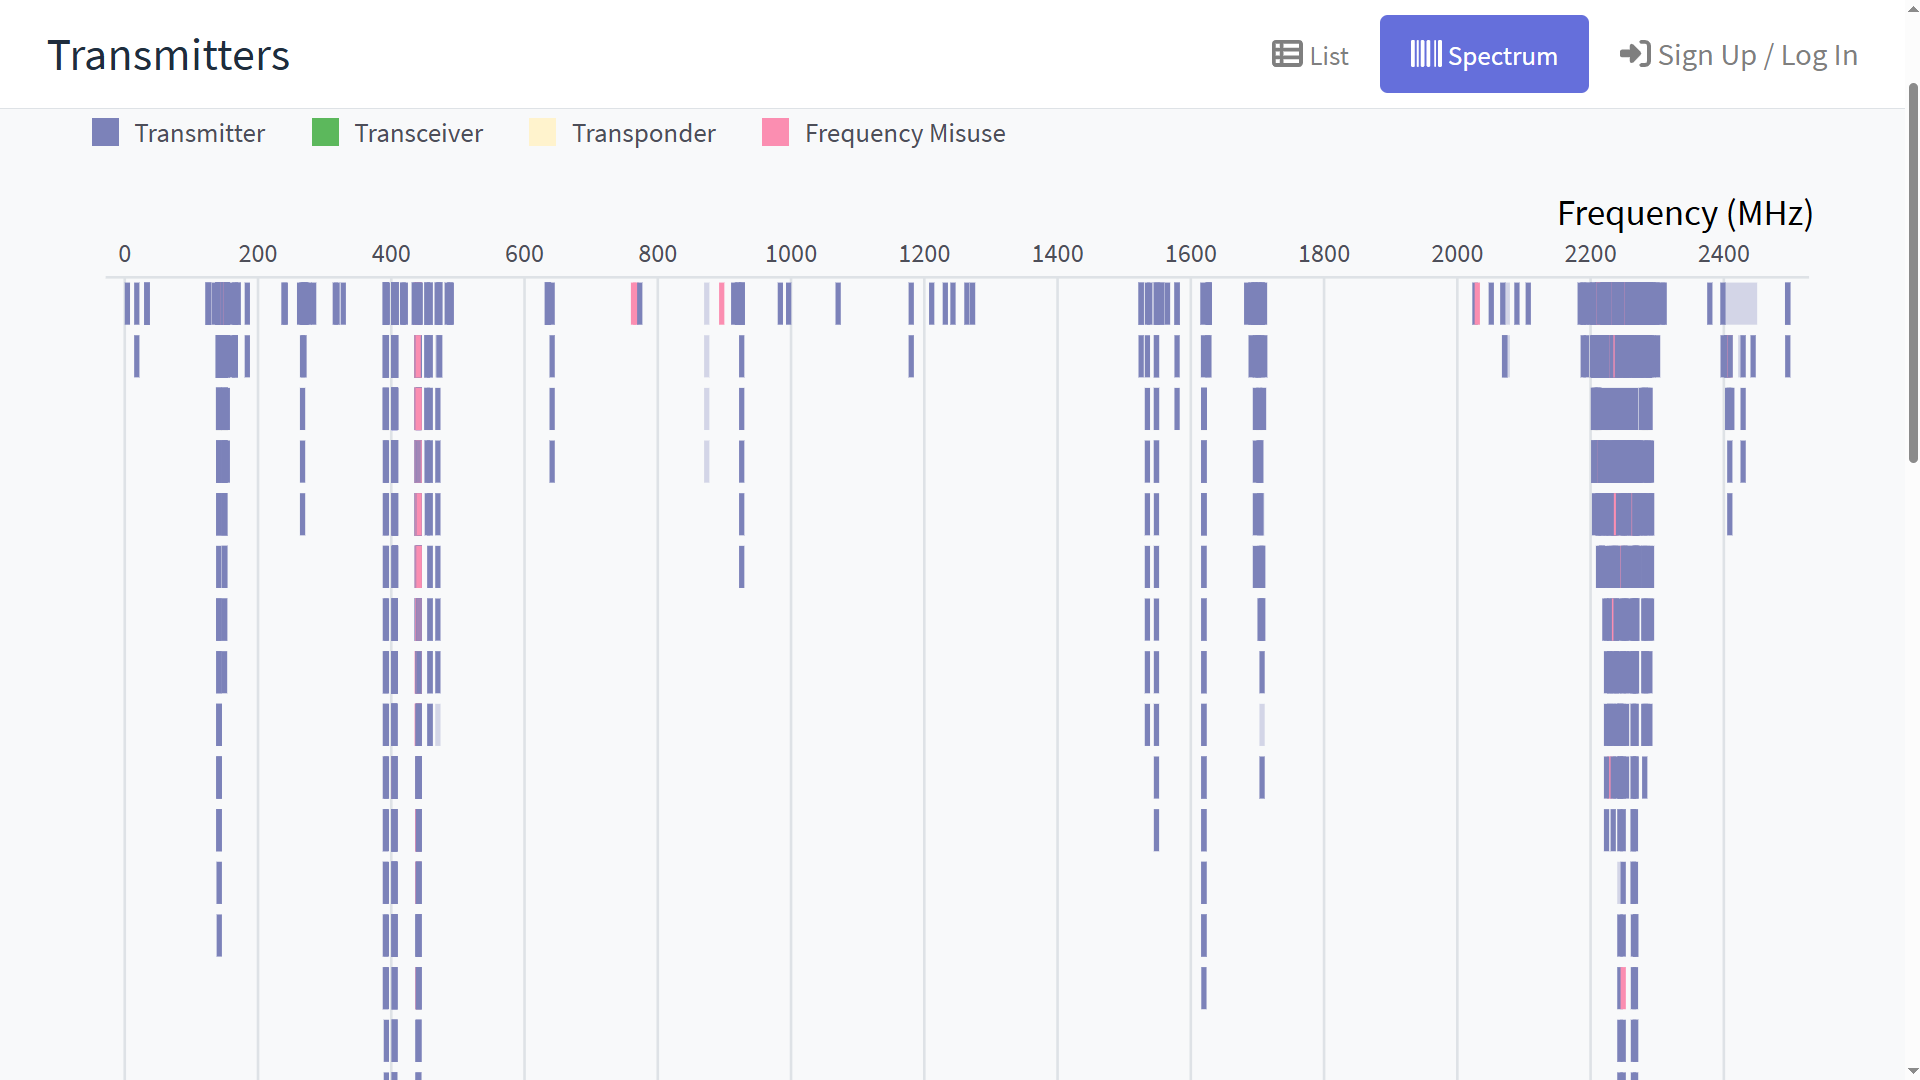
\includegraphics[width=0.8\textwidth]{images/2025-05-22-15-45-18.png}
%  \caption{}
 \end{figure}

\end{frame}

\begin{frame}{amateur frequencies}
  
\begin{figure}
 \centering
 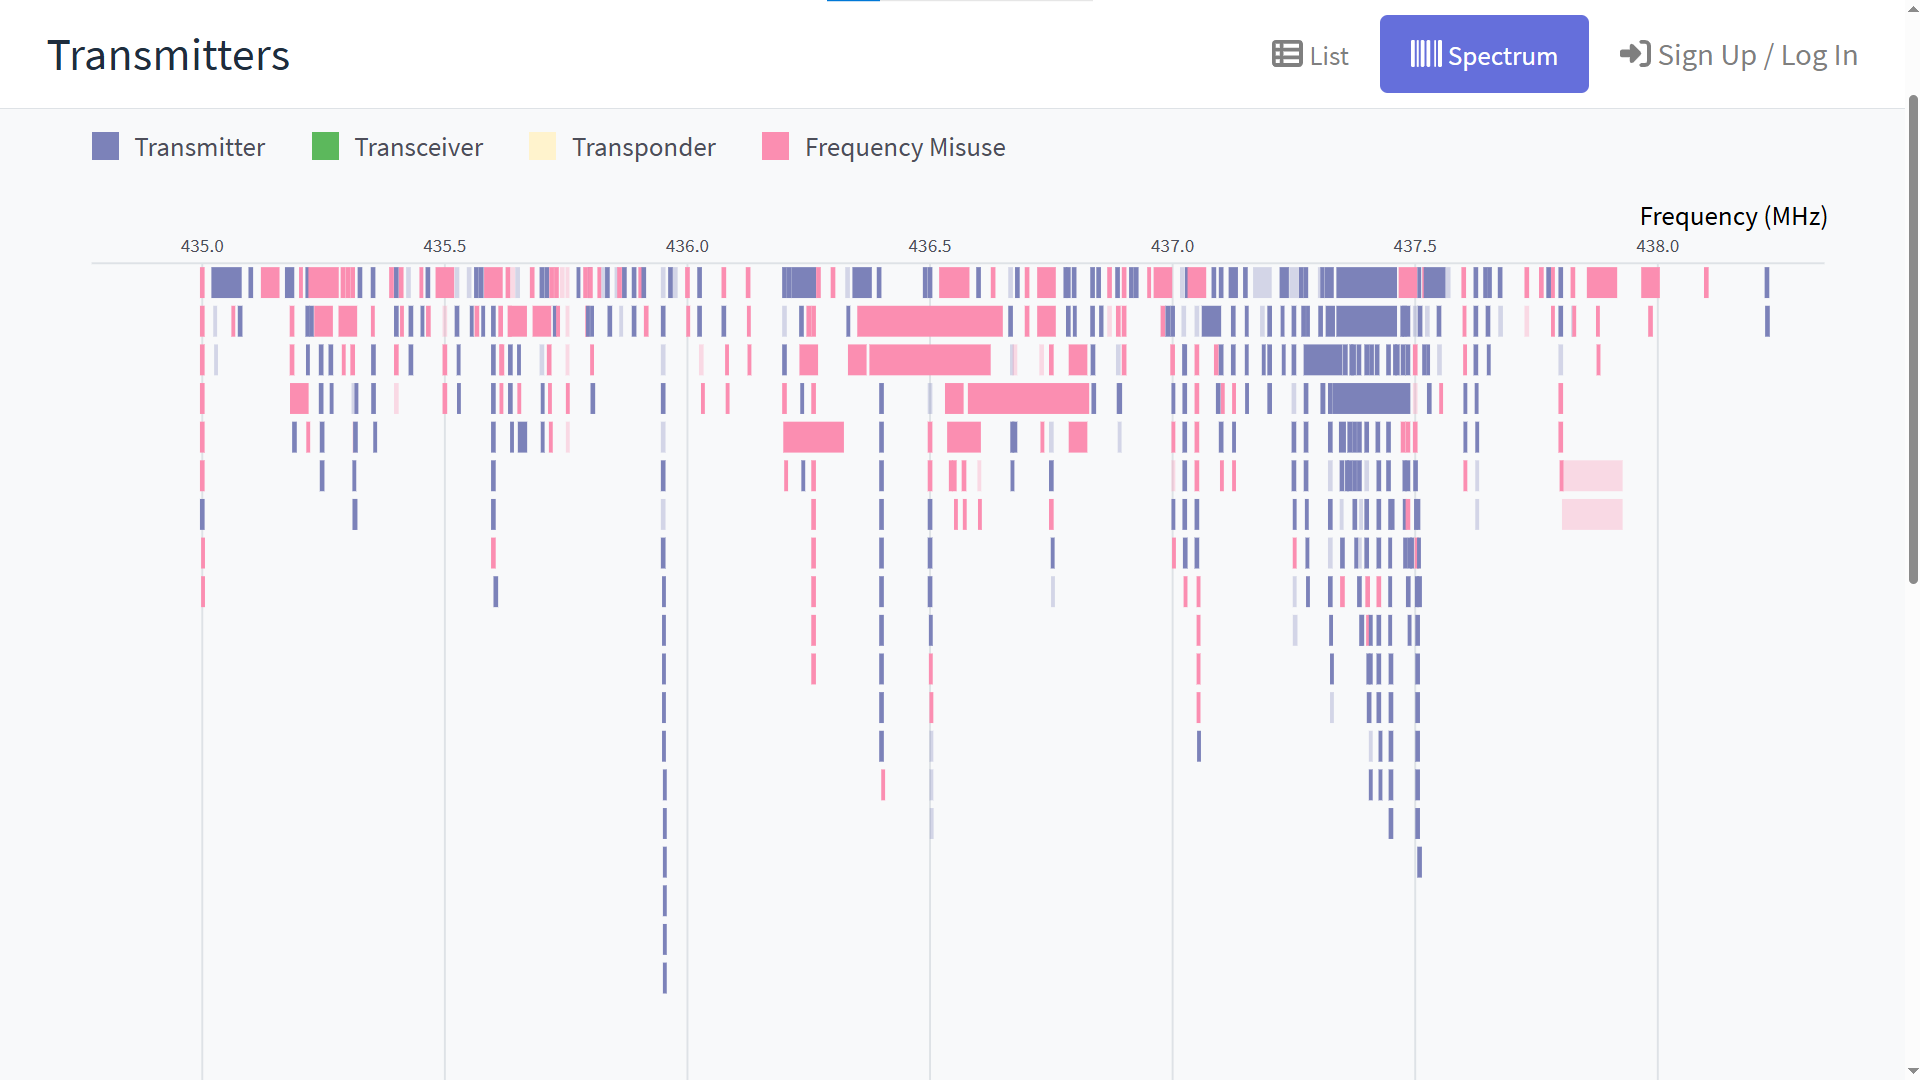
\includegraphics[width=0.8\textwidth]{images/2025-05-22-16-01-18.png}
%  \caption{}
 \end{figure}

\end{frame}

% \begin{frame}{why tho?}{}
  
% \end{frame}

\section{antenna}

% \begin{frame}{antenna}{}

%  % Turnstile antenna schematic in TikZ with top and side views
% % Usage: include this in a LaTeX document with \usepackage{tikz}
% % Turnstile antenna schematic in TikZ with top and side views
% % Usage: include this in a LaTeX document with \usepackage{tikz}
% % Turnstile antenna schematic in TikZ with top and side views
% % Usage: include this in a LaTeX document with \usepackage{tikz}
% \begin{tikzpicture}[scale=0.7, every node/.style={font=\sffamily}, >=latex]
%   % Legend
%   \begin{scope}[xshift=-7cm, yshift=3cm]
%     % Aluminum rod
%     \draw[line width=1pt] (0,0) -- ++(0.5,0) node[right]{Aluminum rod};
%     % PVC tube cylinder symbol
%     \shade[draw=black, top color=gray!30, bottom color=gray!30] (0,-0.5) ellipse (0.25 and 0.1) -- ++(0.5,0) ellipse (0.25 and 0.1) -- cycle;
%     \draw (0,-0.5) ellipse (0.25 and 0.1) (0.5,-0.5) ellipse (0.25 and 0.1);
%     \node at (0.75,-0.5) [right]{PVC tube};
%   \end{scope}

%   % Top View
%   \begin{scope}[xshift=-4cm]
%     % Center feed
%     \draw[fill=black] (0,0) circle (2pt) node[below right] {Feed point};
%     % Aluminum rods
%     \draw[line width=1pt] (-2.5,0) -- (2.5,0) node[midway, above] {Al rod: 3/8 $\lambda$};
%     \draw[line width=1pt] (0,-2.5) -- (0,2.5) node[midway, right] {Al rod: 3/8 $\lambda$};
%     % PVC tubes represented as ellipses
%     \shade[draw=black, top color=gray!30, bottom color=gray!30] (-3.5,0) ellipse (0.3 and 0.1);
%     \shade[draw=black, top color=gray!30, bottom color=gray!30] (3.5,0) ellipse (0.3 and 0.1);
%     \shade[draw=black, top color=gray!30, bottom color=gray!30] (0,-3.5) ellipse (0.1 and 0.3);
%     \shade[draw=black, top color=gray!30, bottom color=gray!30] (0,3.5) ellipse (0.1 and 0.3);
%     \node at (0,-4) {\small (a) Top View};
%   \end{scope}

%   % Side View
%   \begin{scope}[xshift=4cm]
%     % Mast
%     \draw[line width=1pt] (0,-4) -- (0,4) node[above] {Mounting mast};
%     % Feed
%     \draw[fill=black] (0,0) circle (2pt) node[below right] {Feed point};
%     % Aluminum rods
%     \draw[line width=1pt] (0,0) -- (2.5,0) node[above right] {Al rod: 3/8 $\lambda$};
%     \draw[line width=1pt] (0,0) -- (-2.5,0) node[above left] {Al rod: 3/8 $\lambda$};
%     % PVC tubes as gray cylinders (side view)
%     \shade[draw=black, top color=gray!30, bottom color=gray!30] (0,0.5) rectangle (3,1) node[midway, above] {PVC: 1/2 $\lambda$};
%     \shade[draw=black, top color=gray!30, bottom color=gray!30] (0,0.5) rectangle (-3,1) node[midway, above] {PVC: 1/2 $\lambda$};
%     % Support bracket
%     \draw[thick] (0,0) -- ++(-0.5,-0.5) -- ++(0,0.5) node[left] {3D bracket};
%     % Coax feed
%     \draw[->] (0.2,0.2) to[bend left] (1.5,1.5) node[above] {Coax feed};
%     \node at (0,-4.5) {\small (b) Side View};
%   \end{scope}
% \end{tikzpicture}


% \end{frame}

% \begin{frame}{setup}

%   % System block diagram of SatNOGS station in TikZ
% % Usage: include in LaTeX document with \usepackage{tikz}
% \begin{tikzpicture}[scale=0.8, every node/.style={font=\sffamily}, >=latex]
%   % Ground station
%   \draw[fill=gray!40] (0,0) rectangle (2,1);
%   \node at (1,0.5) {Ground Station};

%   % RTL-SDR
%   \draw[fill=blue!40] (3,0) rectangle (5,1);
%   \node at (4,0.5) {RTL-SDR};

%   % Antenna
%   \draw[fill=red!40] (6,0) rectangle (8,1);
%   \node at (7,0.5) {Antenna};

%   % Connections
%   \draw[->] (2,0.5) -- (3,0.5);
%   \draw[->] (5,0.5) -- (6,0.5);

%   % Labels
%   \node at (-1,-1) {SatNOGS Station};

%   \node at (4,-2) {RTL-SDR Dongle};
%   \node at (7,-2) {Antenna};
%   \node at (1,-2) {Ground Station};

% \end{tikzpicture}


% \end{frame}

\begin{frame}{setup}

% System block diagram of SatNOGS station in TikZ
% Improved layout for better visibility on slides
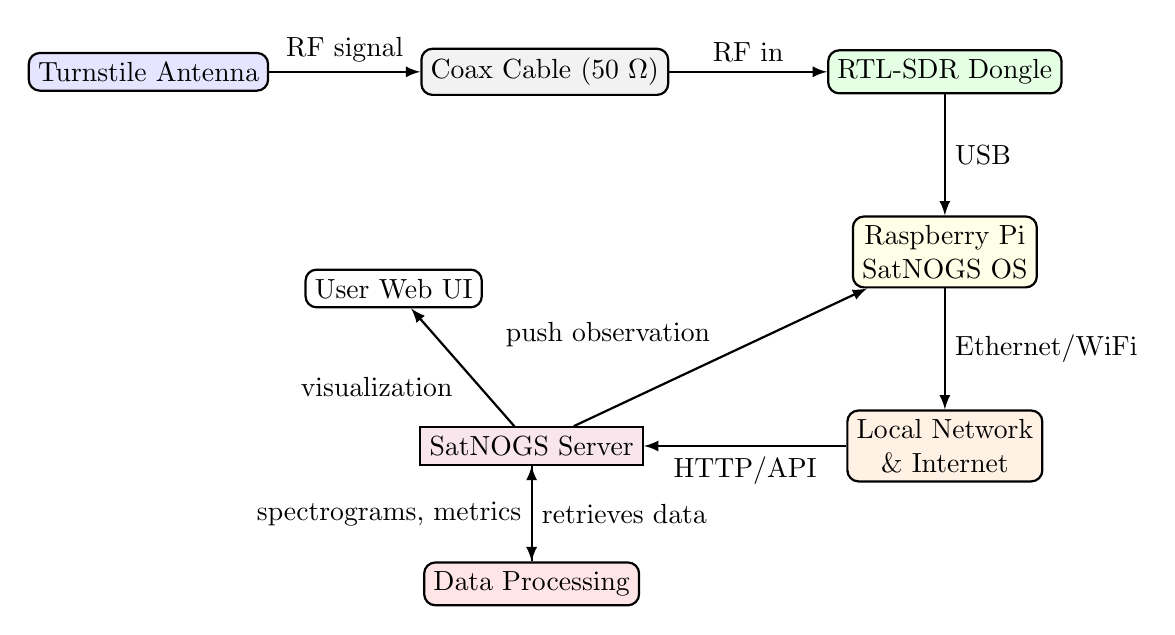
\begin{tikzpicture}[auto, node distance=2cm and 2cm, thick, >=latex, align=center]
  % First row: Signal chain
  \node[draw, rectangle, rounded corners, fill=blue!10] (antenna) at (0,0) {Turnstile Antenna};
  \node[draw, rectangle, rounded corners, fill=gray!10] (coax) at ($(antenna.east)+(3.5,0)$) {Coax Cable (50 \(\Omega\))};
  \node[draw, rectangle, rounded corners, fill=green!10] (sdr) at ($(coax.east)+(3.5,0)$) {RTL-SDR Dongle};
  \node[draw, rectangle, rounded corners, fill=yellow!10] (pi) at ($(sdr.south)+(0,-2)$) {Raspberry Pi\\SatNOGS OS};

  % Second row: Network
  \node[draw, rectangle, rounded corners, fill=orange!10] (network) at ($(pi.south)+(0,-2)$) {Local Network\\ \& Internet};
  \node[draw, rectangle, fill=purple!10] (server) at ($(network.east)-(6.5,0)$) {SatNOGS Server};
  \node[draw, rectangle, rounded corners, fill=red!10] (analysis) at ($(server.south)+(0,-1.5)$) {Data Processing};
  \node[draw, rectangle, rounded corners, fill=white] (ui) at ($(pi.south)+(-7,-0)$) {User Web UI};

  % Connections
  \draw[->] (antenna) -- node{RF signal} (coax);
  \draw[->] (coax) -- node{RF in} (sdr);
  \draw[->] (sdr) -- node{USB} (pi);
  \draw[->] (pi) -- node{Ethernet/WiFi} (network);
  \draw[->] (network) -- node{HTTP/API} (server);
  \draw[->] (server) -- node{retrieves data} (analysis);
  \draw[->] (server) -- node{push observation} (pi);
  \draw[->] (server) -- node{visualization} (ui);
  \draw[->] (analysis) -- node{spectrograms, metrics} (server);

  % Title
  % \node[anchor=north, font=\large\bfseries] at ($(antenna.north)!0.5!(server.north)+(0,1.2cm)$) {SatNOGS Station System Diagram};
\end{tikzpicture}


\end{frame}

\begin{frame}{antenna}

  \begin{columns}
  \column{0.5\textwidth}
  \begin{figure}[!ht]
\centering
\resizebox{0.8\textwidth}{!}{%
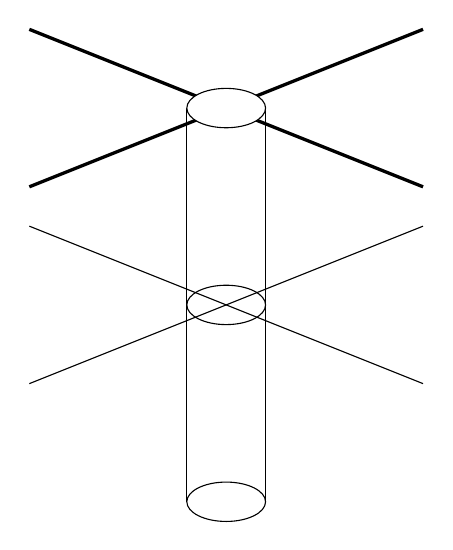
\begin{tikzpicture}
% \tikzstyle{every node}=[font=\LARGE]
\draw (5.75,11.25) -- (5.75,6.25);
\draw (6.75,11.25) -- (6.75,6.25);
\draw  (6.25,8.75) ellipse (0.5cm and 0.25cm);
\draw  (6.25,6.25) ellipse (0.5cm and 0.25cm);
\draw [very thick] (8.75,12.25) -- (3.75,10.25);
\draw [very thick] (3.75,12.25) -- (8.75,10.25);
\draw [fill=white] (6.25,11.25) ellipse (0.5cm and 0.25cm);
\draw (8.75,9.75) -- (3.75,7.75);
\draw (3.75,9.75) -- (8.75,7.75);
\end{tikzpicture}
}%
% \label{fig:my_label}
\end{figure}
\column{0.5\textwidth}

\only<1>{\begin{itemize}
  \item active (upper) rod length: $L_a=\frac{\lambda}{4}=\frac{c}{4f}=16.3$ cm
  \item passive (lower) rod length: $L_p=\frac{\lambda}{2}=\frac{c}{2f}=34.6$ cm
  \item distance between rods: $d=\frac{3\lambda}{8}=\frac{3c}{8f}=25.8$ cm
  \item interference: constructive 
\end{itemize}}
\only<2>{\begin{figure}
 \centering
 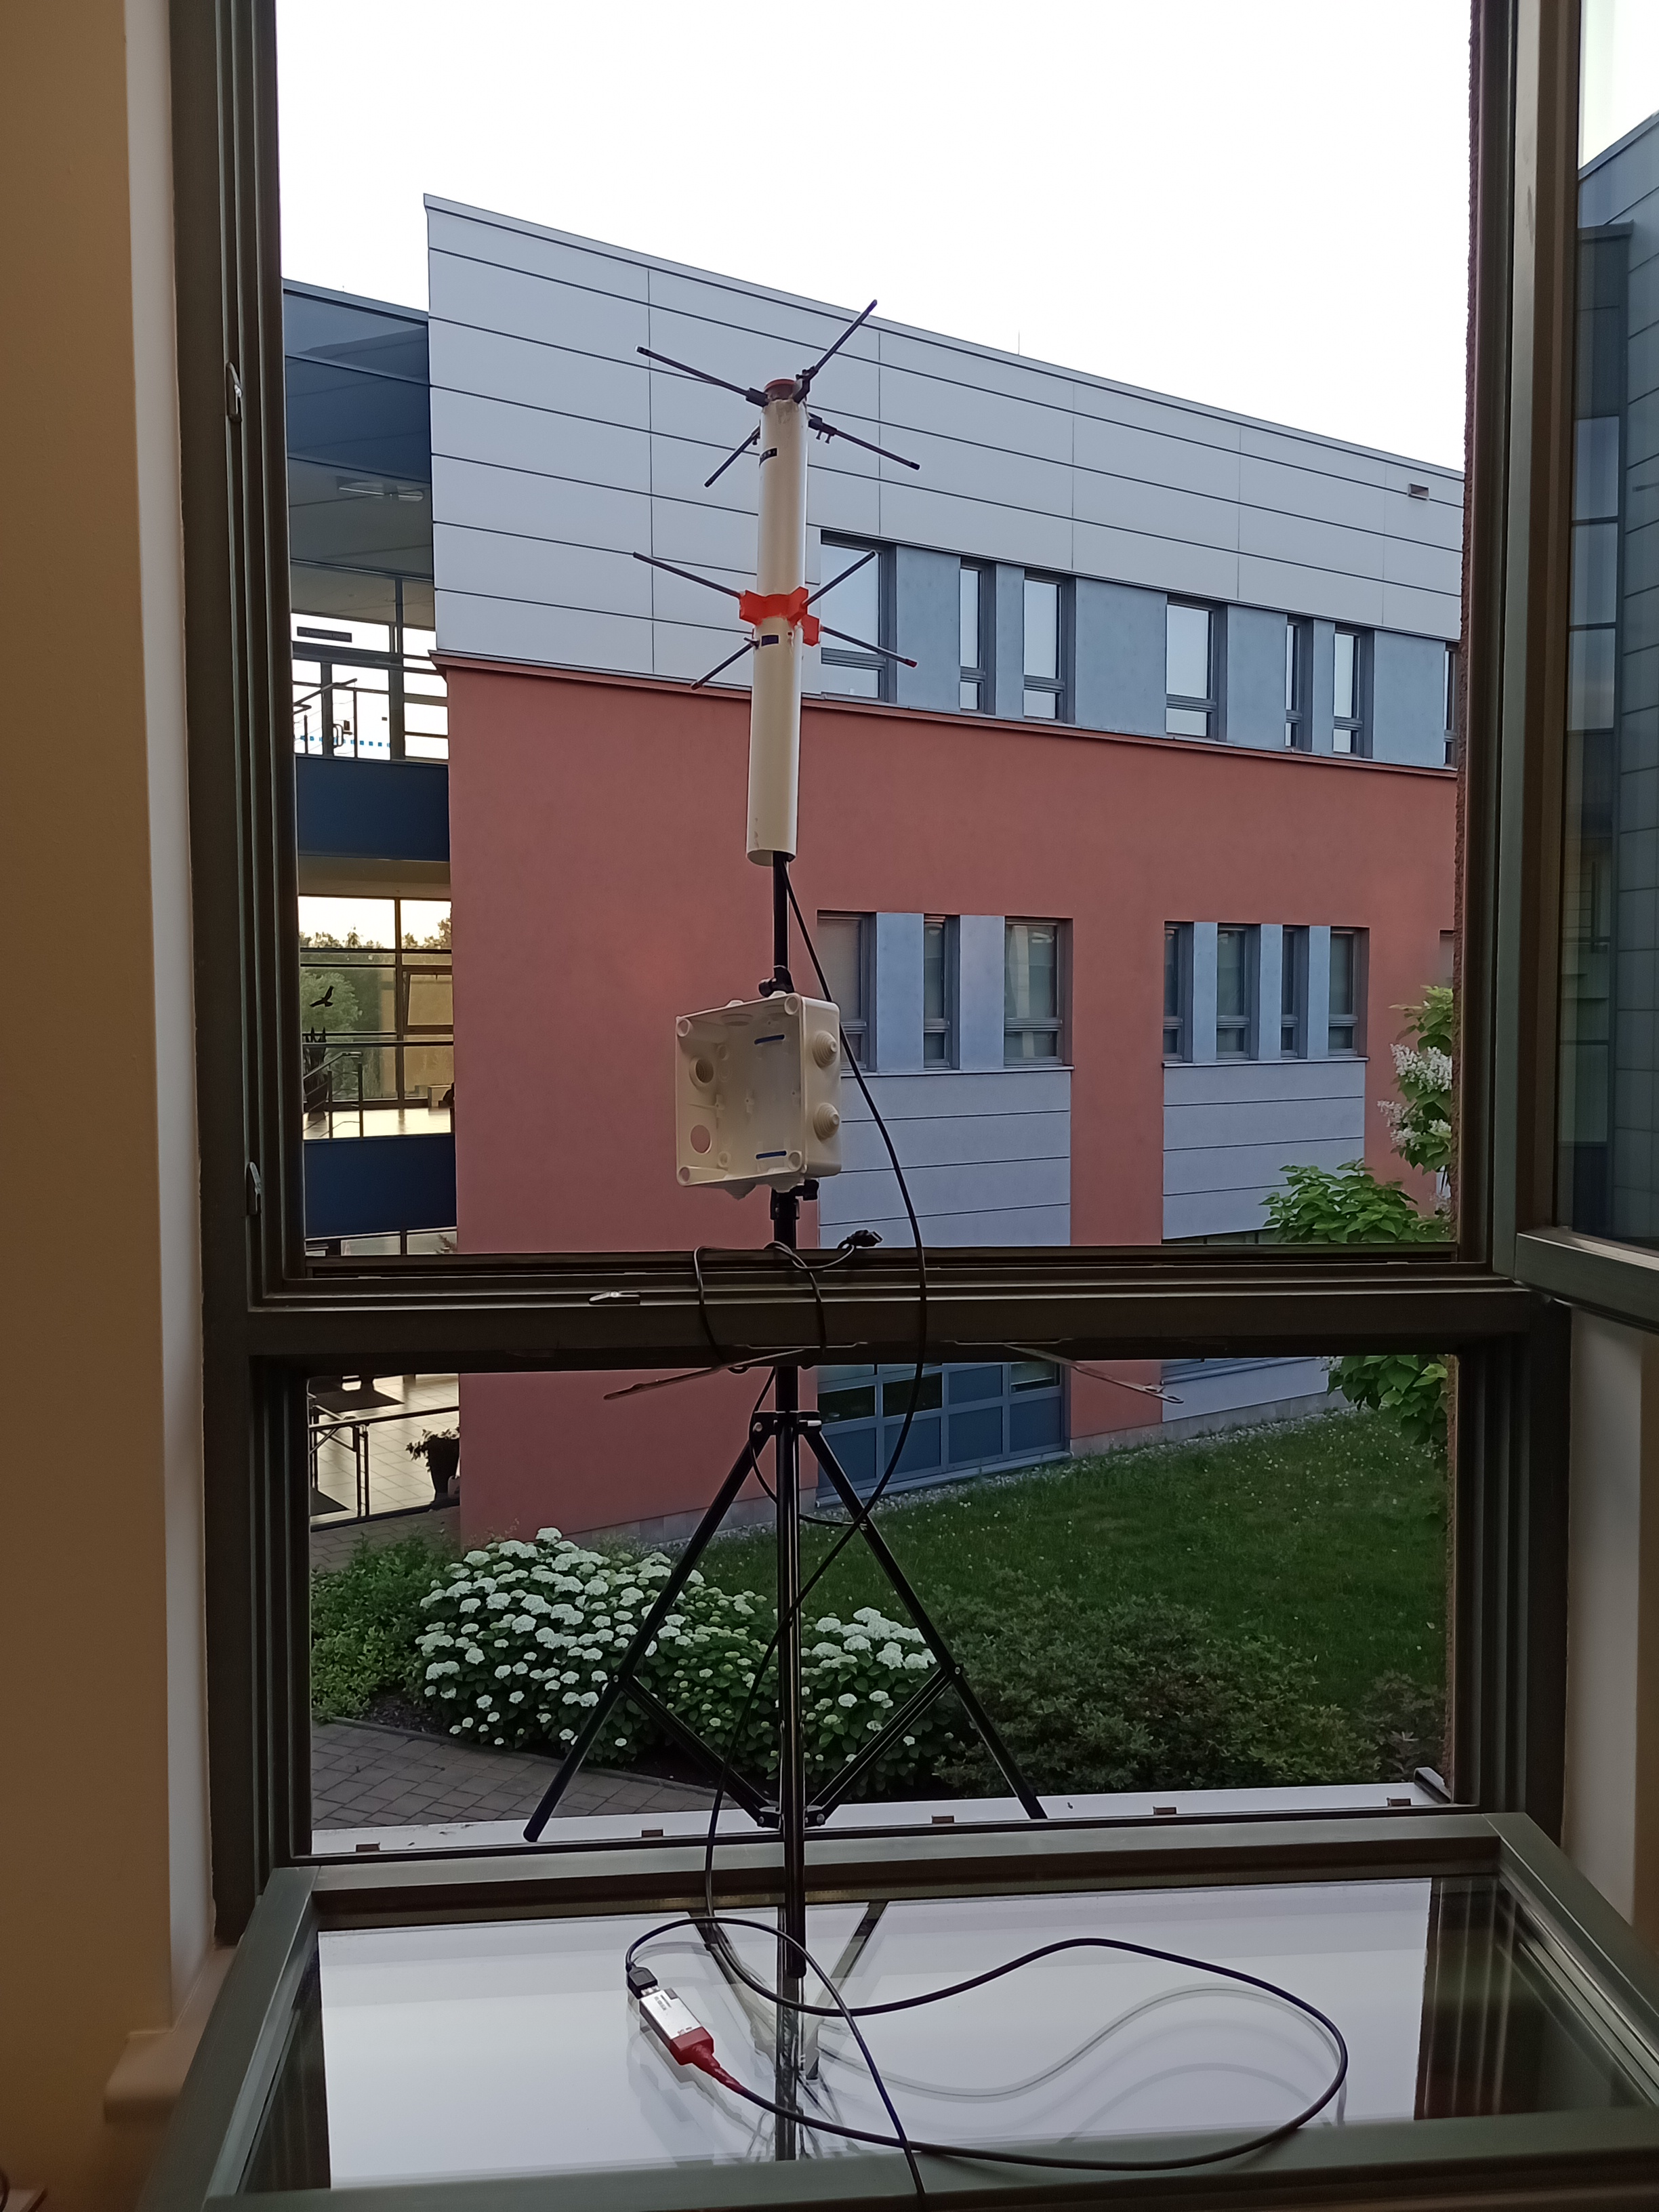
\includegraphics[width=0.7\textwidth]{images/2025-05-22-02-17-05.png}
 \caption{the antenna with RTL-SDR dongle just outside the window}
 \end{figure}}

\end{columns}

\end{frame}

\begin{frame}{sdr + computer}{}

  \begin{columns}
  \column{0.5\textwidth}
  \begin{figure}
 \centering
 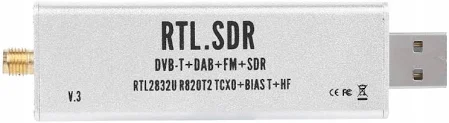
\includegraphics[width=0.9\textwidth]{images/2025-05-23-01-09-08.png}
 \caption{rtl-sdr dongle}
 \end{figure}
\column{0.5\textwidth}
\begin{figure}
 \centering
 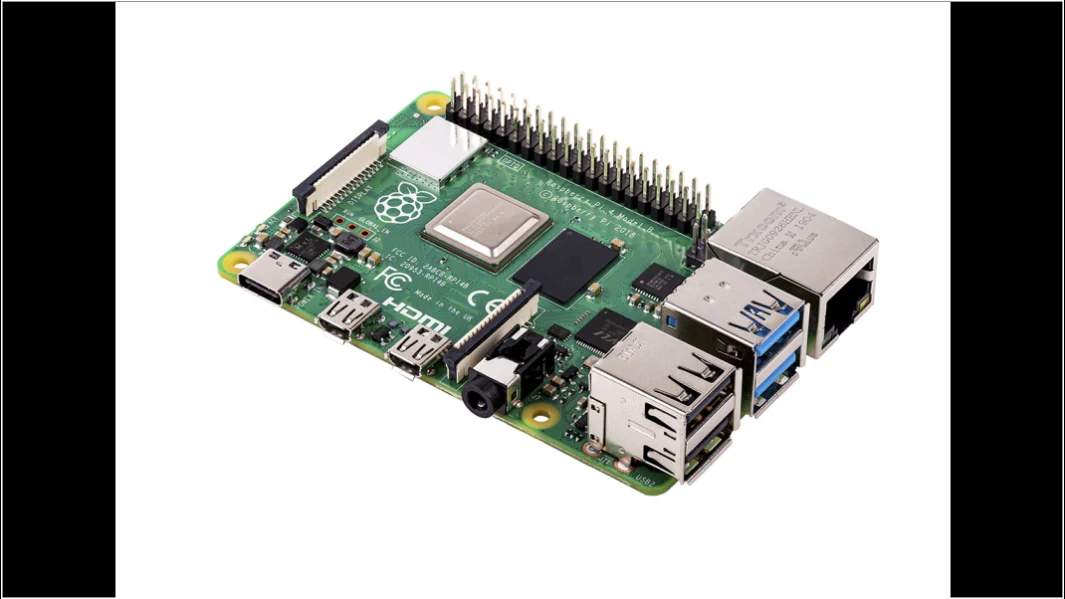
\includegraphics[width=0.9\textwidth]{images/2025-05-23-01-10-57.png}
 \caption{raspberry pi}
 \end{figure}
  \end{columns}
  
\end{frame}


\section{satnogs}

\begin{frame}{satnogs: concept}
  \begin{figure}
 \centering
 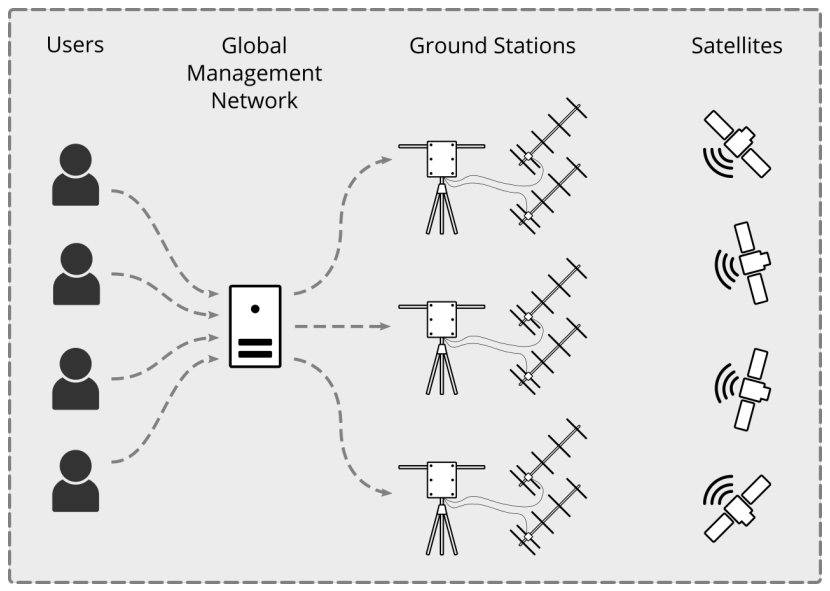
\includegraphics[width=0.5\textwidth]{images/2025-05-22-16-52-43.png}
 \caption{overall view of satnogs (Satellite Network Open Ground Stations) concept}
 \end{figure}
\end{frame}

\begin{frame}{satnogs network}

  \begin{figure}
 \centering
 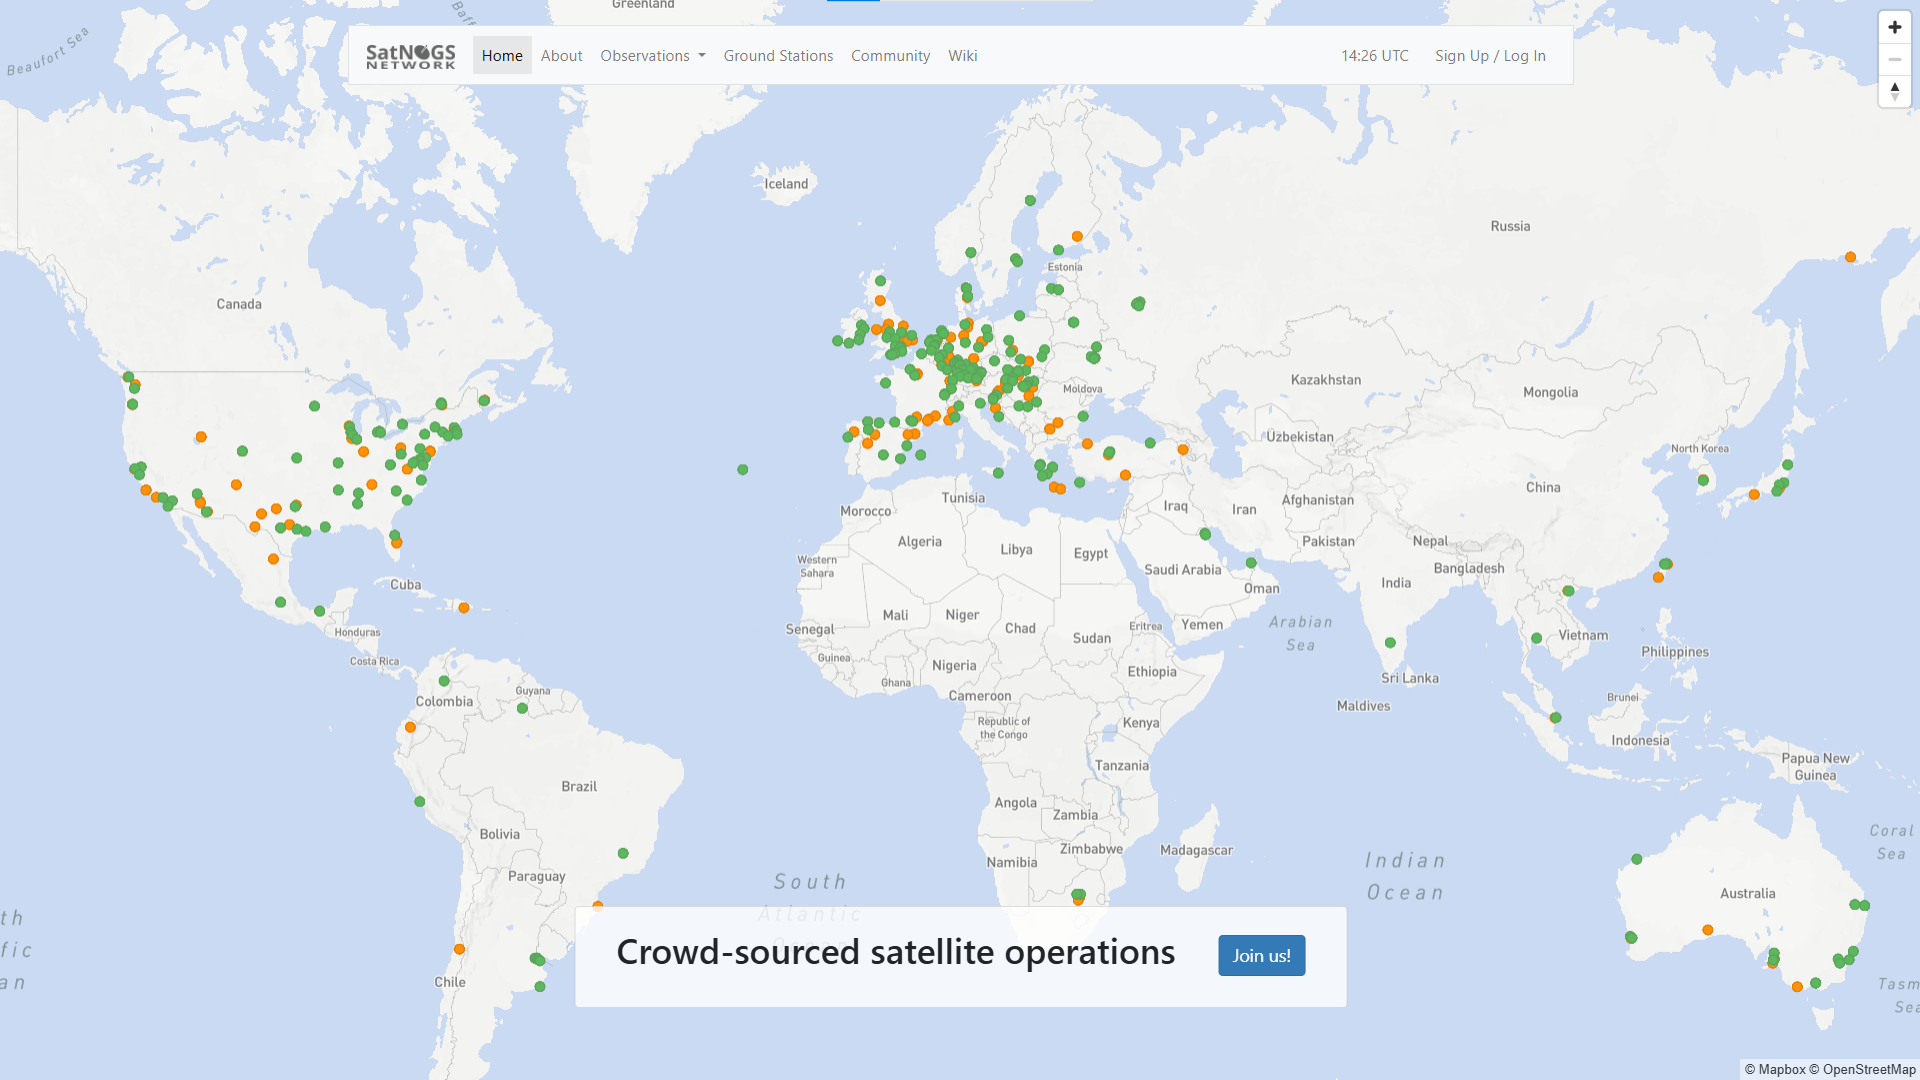
\includegraphics[width=0.9\textwidth]{images/2025-05-13-16-27-13.png}
%  \caption{}
 \end{figure}
  
\end{frame}

\section{observations}

\begin{frame}{good observations I }{}
\begin{columns}

\column{0.5\textwidth}
% \begin{figure}
%  \centering
%  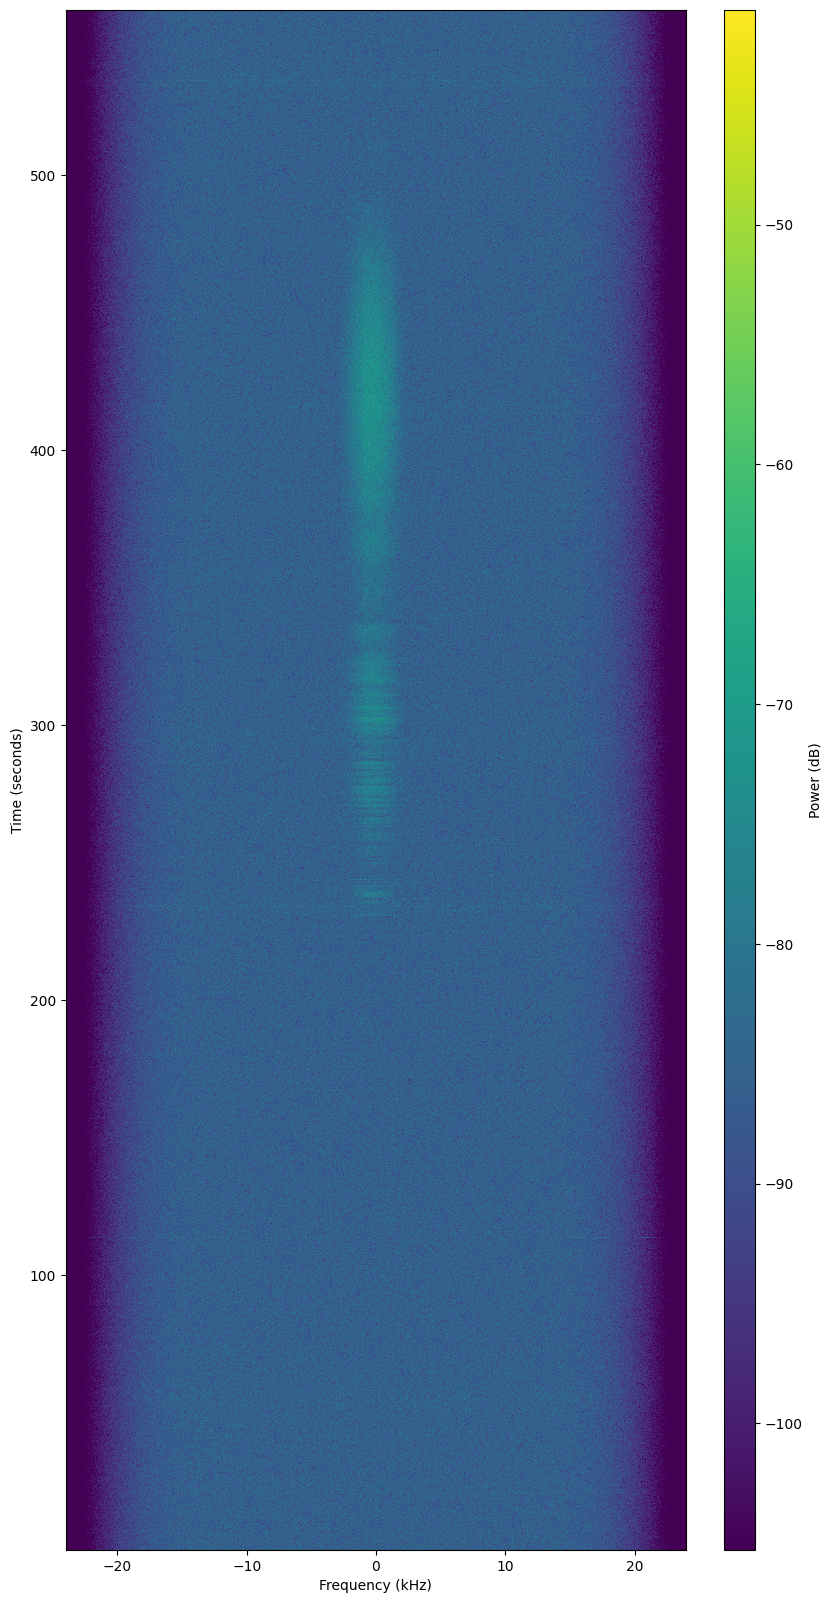
\includegraphics[width=0.5\textwidth, angle=270]{images/2025-05-23-11-18-50.png}
%  \caption{satellite 44886, transmitter: mode U}
%  \end{figure}
\begin{figure}
 \centering
 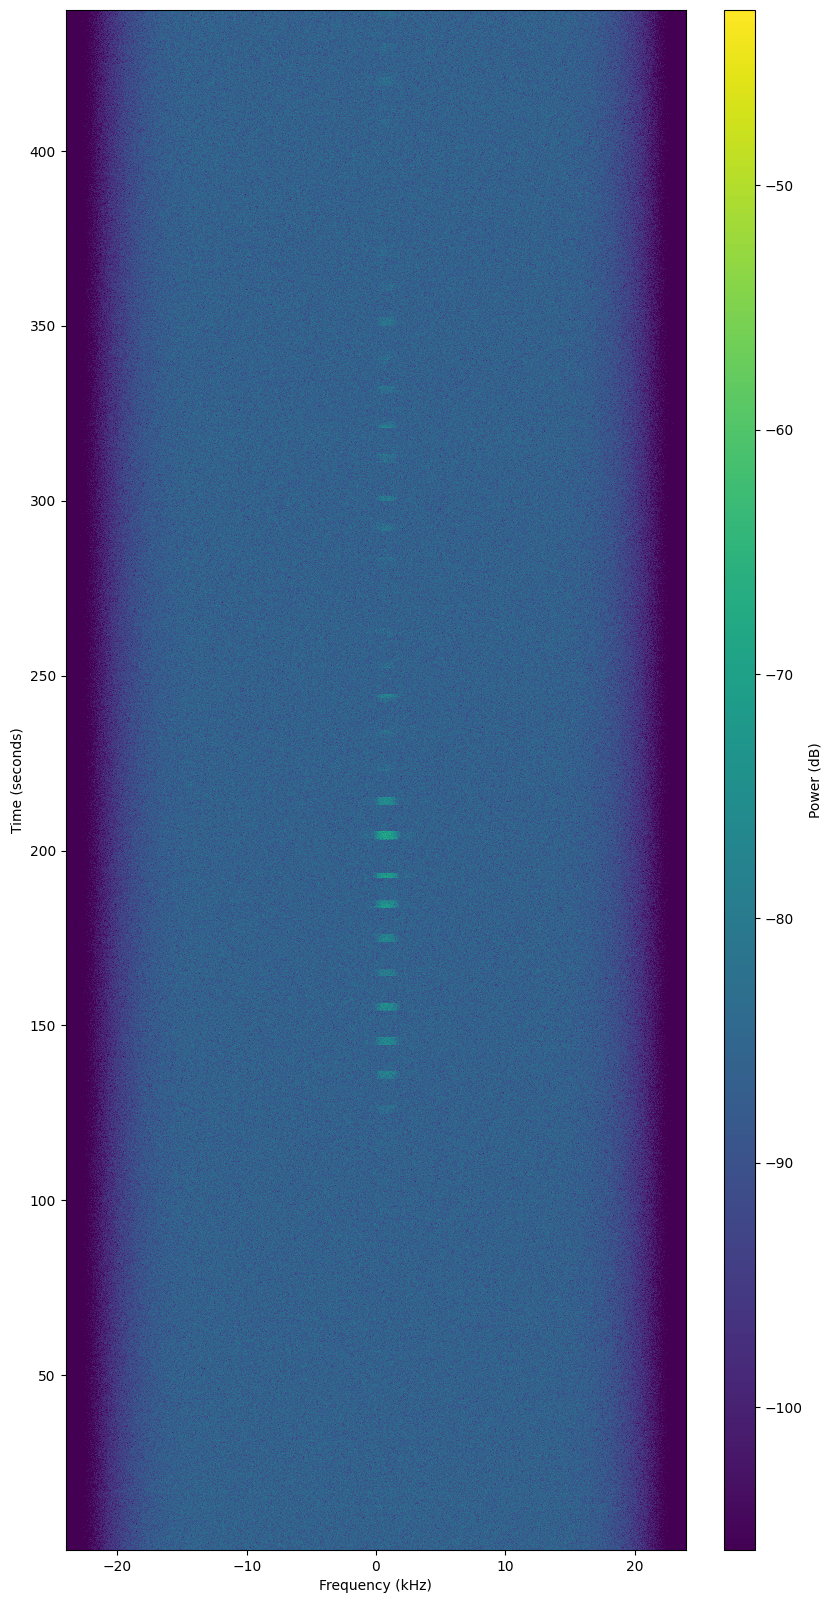
\includegraphics[width=0.6\textwidth, angle=270]{images/2025-05-23-11-22-57.png}
 \caption{satellite DhabiSat, transmitter: BPSK}
 \end{figure}
\column{0.5\textwidth}
\begin{figure}
 \centering
 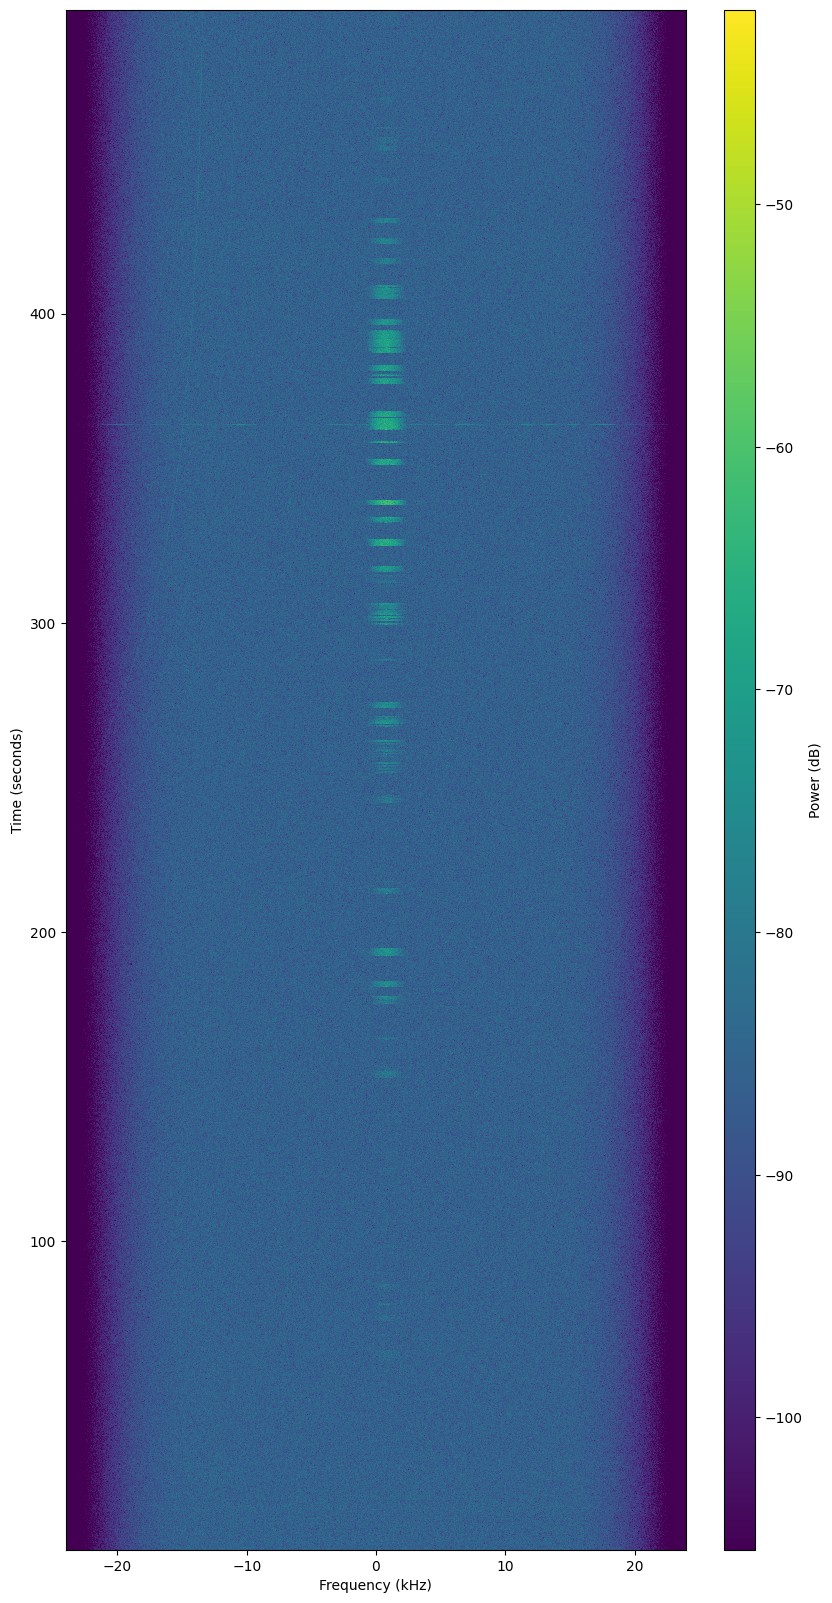
\includegraphics[width=0.6\textwidth, angle=270]{images/2025-05-23-11-19-51.png}
 \caption{satellite SITRO-AIS-9, transmitter: GMSK}
 \end{figure}
\end{columns}
\end{frame}
\begin{frame}{good observations II}{}

\begin{columns}

\column{0.5\textwidth}
\begin{figure}
 \centering
 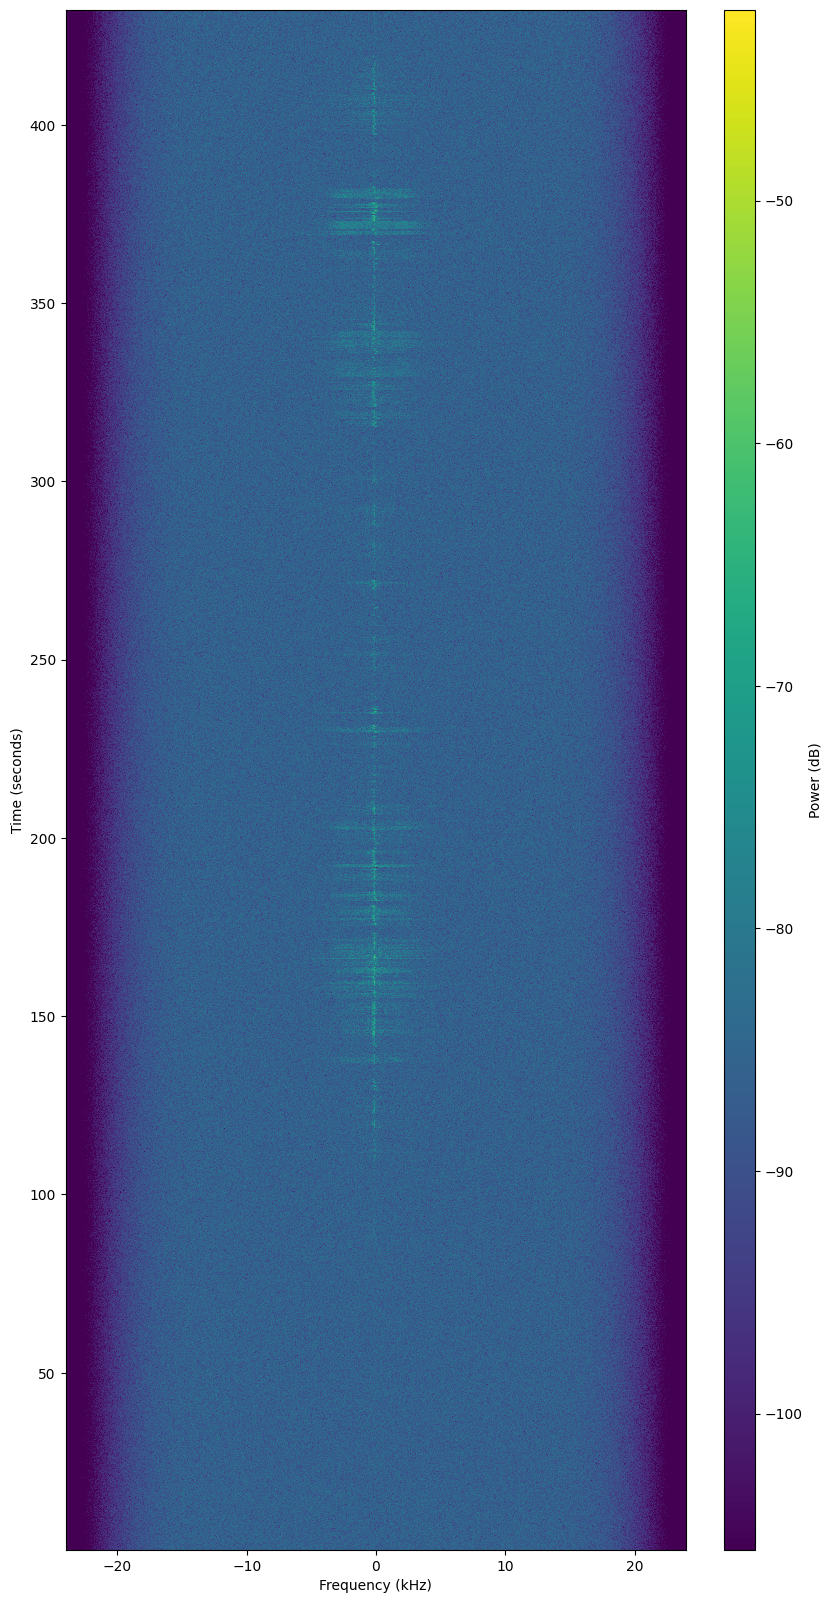
\includegraphics[width=0.6\textwidth, angle=270]{images/2025-05-23-11-38-44.png}
 \caption{satellite ISS, transmitter V/U FM}
 \end{figure}
\column{0.5\textwidth}
\begin{figure}
 \centering
 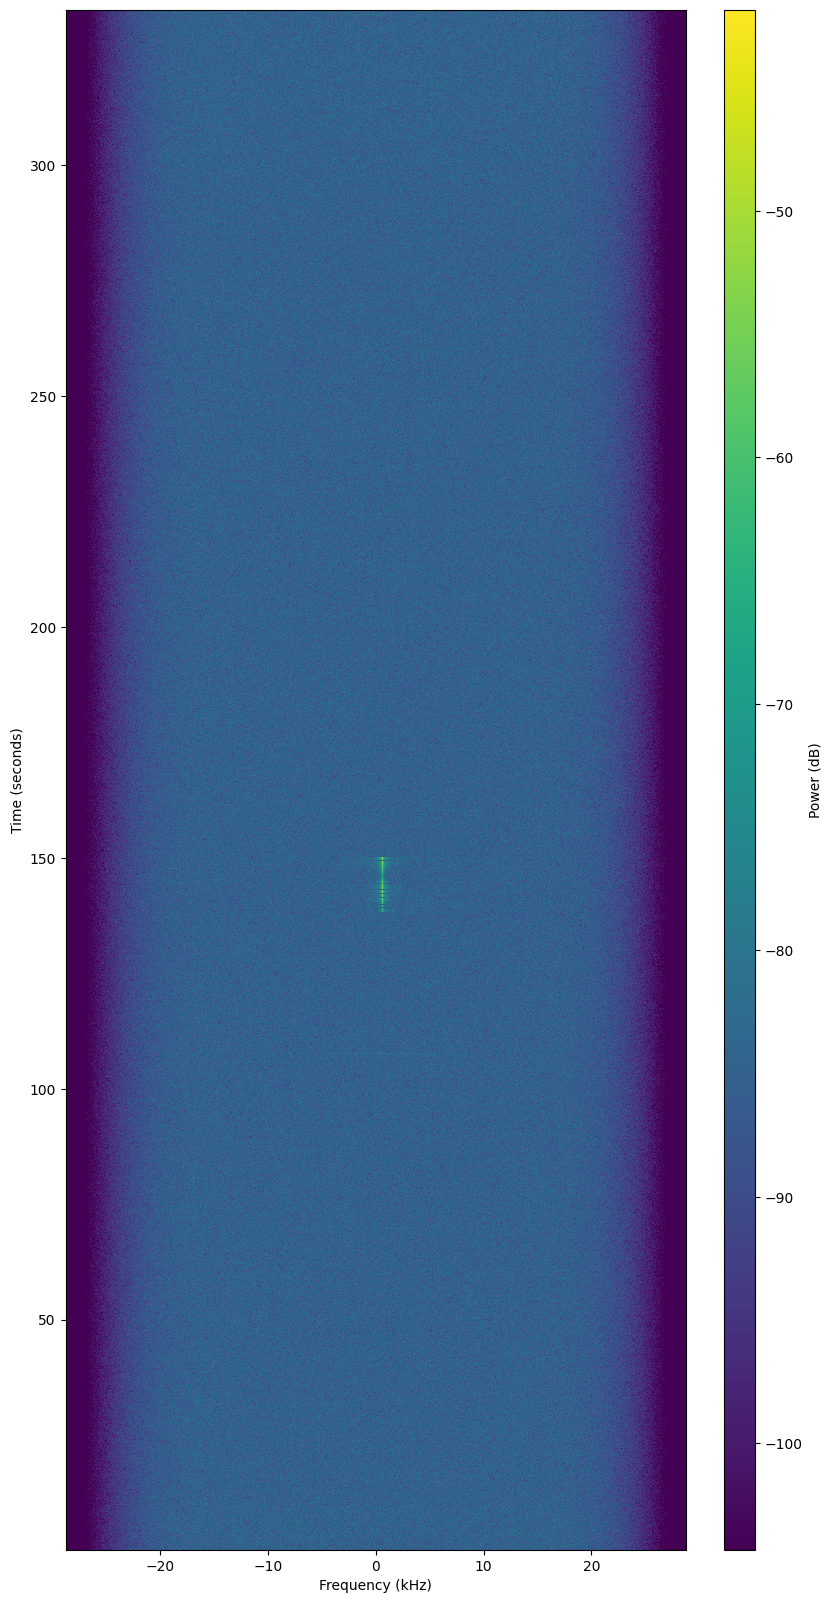
\includegraphics[width=0.6\textwidth, angle=270]{images/2025-05-23-11-47-10.png}
 \caption{satellite Reaktor Hello World, transmitter: GFSK}
 \end{figure}
\end{columns}
\end{frame}

\begin{frame}{decoding signal}{}
\begin{figure}
 \centering
 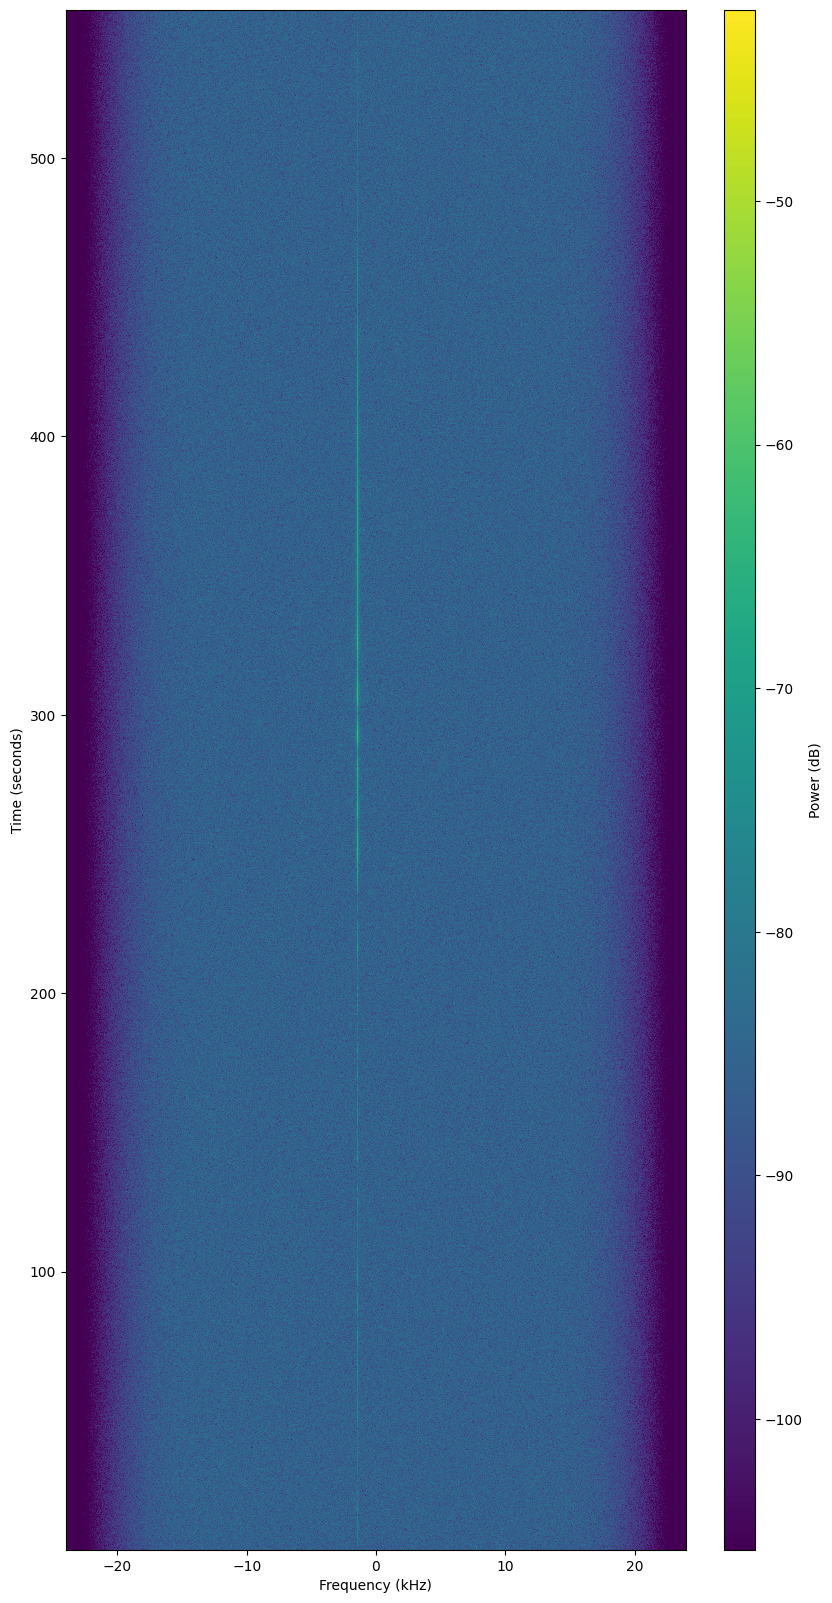
\includegraphics[width=0.3\textwidth, angle=270]{images/2025-05-23-11-31-29.png}
 \caption{satellite: LUSAT, transmitter: TLM}
 \end{figure}
\begin{figure}
 \centering
 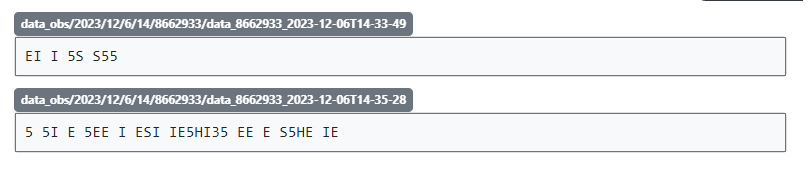
\includegraphics[width=0.7\textwidth]{images/2025-05-23-11-32-15.png}
%  \caption{}
 \end{figure}
\end{frame}

\begin{frame}{bad observations}{}

\begin{columns}

\column{0.5\textwidth}
\begin{figure}
 \centering
 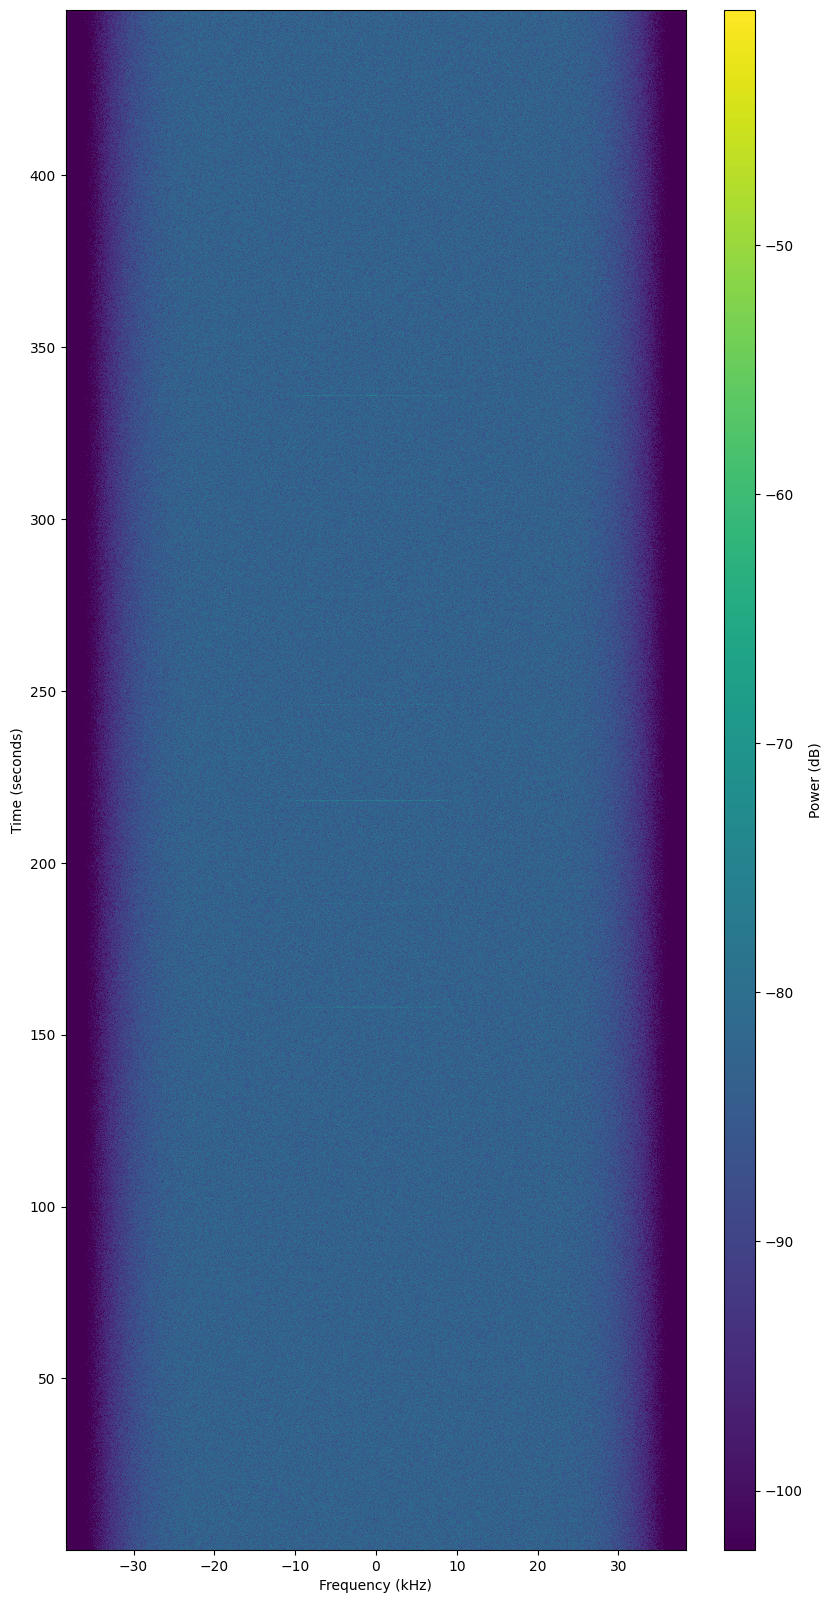
\includegraphics[width=0.6\textwidth, angle=270]{images/2025-05-22-21-10-28.png}
 \caption{bad result -- no signal}
 \end{figure}
\column{0.5\textwidth}
\begin{figure}
 \centering
 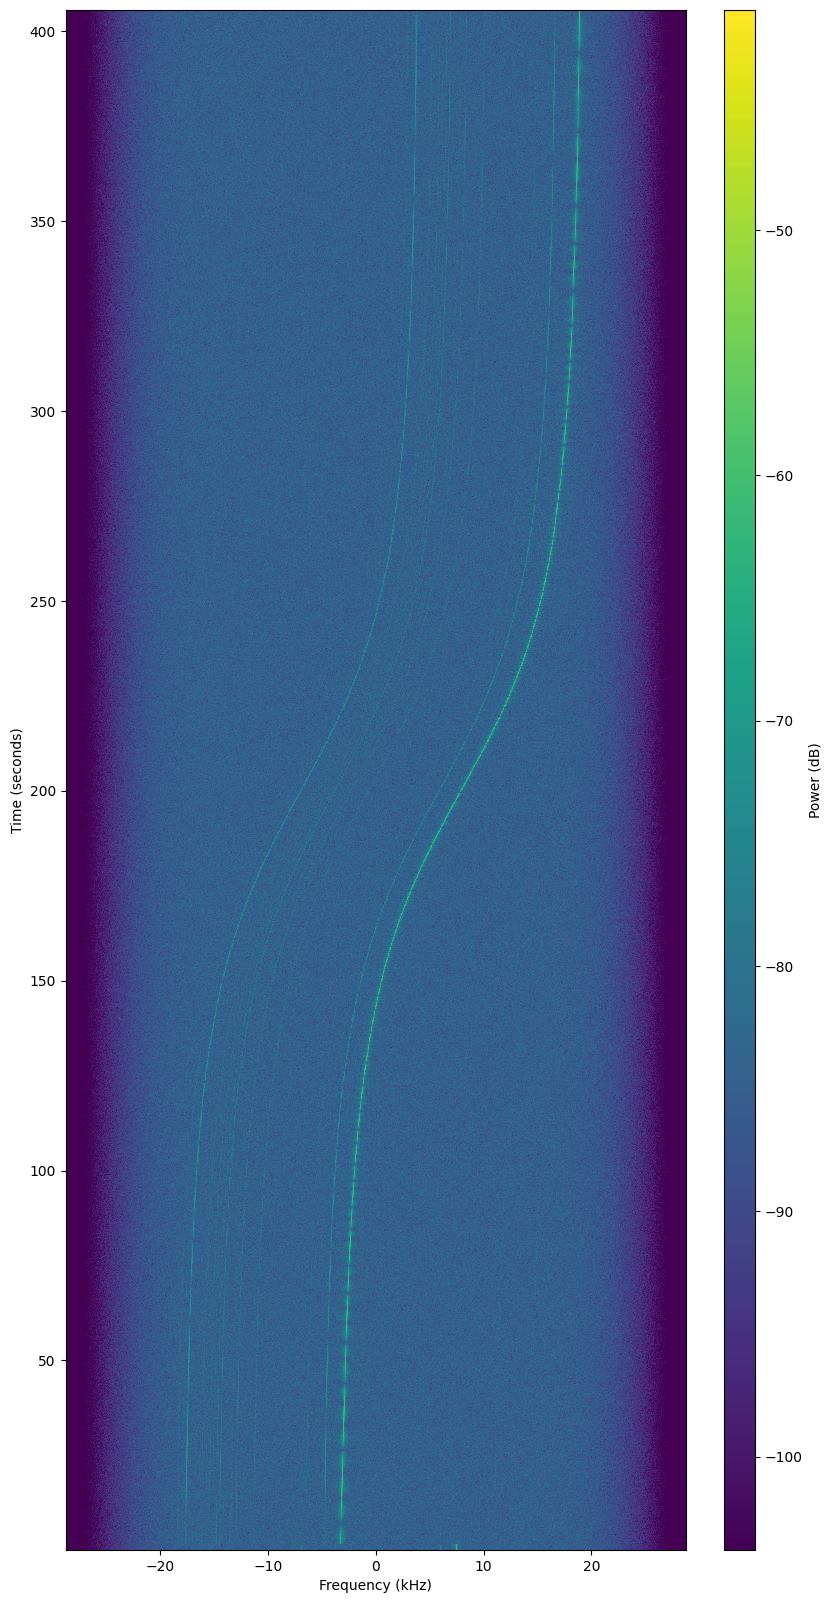
\includegraphics[width=0.6\textwidth, angle=270]{images/2025-05-22-21-03-20.png}
 \caption{also a bad result -- tangent-like signal means terrestrial noise}
 \end{figure}
\end{columns}
\end{frame}


\begin{frame}

  \begin{columns}
\column{0.6\textwidth}
  
\begin{figure}
 \centering
 
\includegraphics[width=0.85\textwidth]{images/2025-05-13-15-25-41.png}
%  \caption{}
 \end{figure}

 \centering project co-funded by Garage of Complexity
\column{0.4\textwidth}
\begin{figure}
 \centering
 
\includegraphics[width=0.9\textwidth]{images/2025-05-23-01-45-08.png}
%  \caption{}
 \end{figure}
  \end{columns}
\end{frame}

\begin{frame}{bibliography}{}
  \nocite{*}
  \printbibliography[heading=none]
\end{frame}

\begin{frame}{}{}
  \vspace{-1cm}
\begin{figure}
\centering
  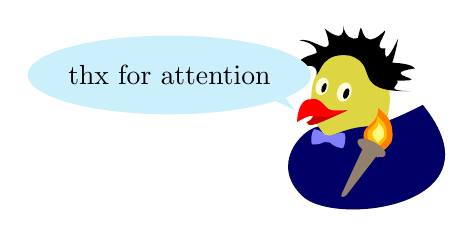
\begin{tikzpicture}
    \duck[parrot, body=gray!30!yellow, head=gray!30!yellow, bill=red, torch=gray!70!brown, tshirt=blue!40!black, ribbon=gray, bowtie=blue!50!white, crazyhair=black]
    %\addwater{blue!50!cyan}
    \fill[cyan!20!white] (-1.4,1.8) ellipse (1.8 and 0.5);
\fill[cyan!20!white] (-0.2,1.54) -- (0.2,1.35) -- (0.0,1.6) -- cycle;
\node at (-1.4,1.8) {thx for attention};
  \end{tikzpicture}
  \end{figure}


  
  \begin{figure}
  \centering
        
\includegraphics[height=0.3\linewidth]{images/2025-05-13-15-25-41.png}\\
  {\scriptsize \url{https://github.com/falcotinnunculus/przezrocza/blob/wladca/sempowisko2025/sempo.pdf}}

  \end{figure}
\vspace{-5.3cm}
\transparent{0.7}
  \begin{figure}
      \centering
      \qrcode[height=0.3\textwidth]{https://github.com/falcotinnunculus/przezrocza/blob/wladca/sempowisko2025/sempo.pdf}
      % \caption{Caption}
      % \label{fig:enter-label}
  \end{figure}
\end{frame}


\end{document}